%--------------------------------------
%	Chapter 4. ML Hit-Pair Predictor
%--------------------------------------

%\doublespacing
%\newpage
%\setcounter{section}{3}
%\section{The Compressed Pattern Space}
\chapter{Machine Learning Hit-Pair Predictor} 
\label{chapter-4}
% DONE


% This study was conducted in order to speed up the track seeding stage and reduce CPU time in the ATLAS fast tracking trigger algorithm.

When constructing graph networks for track reconstruction, one must first consider the ability to identify compatible hit connections to build graph edges. A beneficial step towards enhancing this process is to reduce the number of fake edges constructed and hence increase the accuracy in predicting such compatible hit-pairs. As future upgrades to particle detectors will lead to significant increases in hit occupancy, this will be problematic for silicon tracking detectors. Therefore, it is essential that resource use is also considered, whilst maintaining the capability to reconstruct tracks with minimal efficiency loss. This chapter presents a methodology to accomplish such a task. This work is presented in the Journal of Physics: Conference Series \cite{Lad_2023} and is implemented in the optimisation of the HLT ID track seeding software for ATLAS Run-3 and beyond \cite{Grandi:2728111, Long:2813981}. Section \ref{measurement-to-track-association} presents the development of a ML-based algorithm to predict if a pair of hits belongs to the same track given input hit features, namely cluster width and inverse track inclination. The implementation of the trained predictor in the form of Look-Up Tables (LUTs) is presented in Section \ref{application-of-hit-pair-predictor}. Performance results, including tracking efficiency and speed-up factor are measured using simulated data and discussed.


\section{Measurement to Track Association}
\label{measurement-to-track-association}

\subsection{Data Exploration and Feature Extraction}

Seeds constructed at the combinatorial stage of ATLAS tracking software designed for the Run-2 geometry were used to extract hit-pairs to form a training dataset. Monte Carlo (MC) $t\bar{t}$ event samples with centre-of-mass energy $\sqrt{s}$ = 13 TeV at mean pile-up interaction multiplicity $\langle \mu \rangle$ = 80 were used. Top quark simulation is often used for developing algorithms in tracking due to its many possible final states including electron, muon and $\tau$ leptons, as well as hadrons. Due to the presence of pile-up, the multiplicity of constructed seeds is high. A larger proportion of fake seeds will be naturally present, so that $t\bar{t}$ with pile-up provides a good description of the environment in high luminosity conditions.

The training is focused on pixel detector layers, being closest to the beamline and having highest hit occupancy. An illustration of a seed in the ID pixel layers is shown in Figure \ref{fig:triplet-illustration}. The input seeds are triplets of space-points which are deconstructed into pairs of doublets sharing a common middle space-point. For each seed, the inner doublet (defined as hit-pair 1 and 2) and outer doublet (defined as hit-pair 2 and 3) are extracted. The total number of pixel barrel and pixel endcap hit-pairs extracted, and were subsequently used as training samples presented to the classifier, were 365,937 and 18,537 respectively. For each hit-pair, the absolute inverse slope of the track, $|\cot(\theta)|$, is calculated using $r$-$z$ coordinates and used as an input feature for training. $\theta$ is the angle of inclination of a hit-pair with respect to the $z$ axis. The longitudinal pixel cluster width, $w_{\eta}$, measured in the $\eta$ direction was also extracted, where $\eta$ is defined in Eq. \ref{eq:pseudorap}. The MC-generated data in the [$|\cot(\theta)|$, $w_{\eta}$] phase space behaves as a set of 1-dimensional distributions, each with discrete $w_{\eta}$. This is a direct result of charge deposition over a grid of pixels in the simulated pixel modules. The geometry of pixel modules are subdivided into majority \textit{standard} pixels of width 400 $\mu$m and 10\% of \textit{long} pixels of width 600 $\mu$m. The long pixels are responsible for covering the gap between the front-end chips on the modules and provide full coverage \cite{pixel-module-dimensions}. Hence, the discrete cluster widths are observed to be increasing in increments of 200 $\mu$m. This characteristic is exploited to form an ensemble of predictors. 

The MC truth information for seeds and their corresponding hit-pairs were extracted from ATLAS tracking software and used as targets in training. Doublets where both hits belong to the same truth track were labeled as truth 1 (correct hit association). Conversely, doublets where both hits do not belong to the same truth track were labeled as truth 0 (incorrect hit association). Hit-pairs for the pixel barrel and endcap are handled separately in order to build regional classifiers. Hit-pairs located in the transition region of the ID belonging to both barrel and endcap layers are automatically assigned to the barrel classifier. This decision was made such that seeds which would be rejected in the barrel would differ from seeds rejected in the endcap, hence the classifiers would cover a wide proportion of fakes. Therefore the location and track inclination of the innermost hit is considered and the hit-pair is assigned to the corresponding classifier. However, the handling of these doublets can be improved. The same methodology was used for both the pixel barrel and endcap, and are presented in Section \ref{section:classifier-dev} and \ref{application-of-hit-pair-predictor}.

% For seeds where one doublet's hits is completely located in the barrel i.e. both hits are barrel-barrel or completely located in the endcap i.e. both hits are endcap-endcap, and the other doublet in the seed is in the transition region (i.e. barrel-endcap), we look at the location of the middle spacepoint in the seed to determine which regional classifier this data should end up with. i.e. if the middle spacepoint is in the barrel and the outer spacepoint is in the endcap, then this data feeds into the barrel classifier. if the middle spacepoint is in the endcap and inner spacepoint is in the barrel, then this data feeds into the endcap classifier. 

% Maybe this is a flaw/limitation of how the transition region data between barrel and endcap are handled, and really this data should be included in both the barrel and endcap classifiers.



\begin{figure}[!htbp]
\centering
    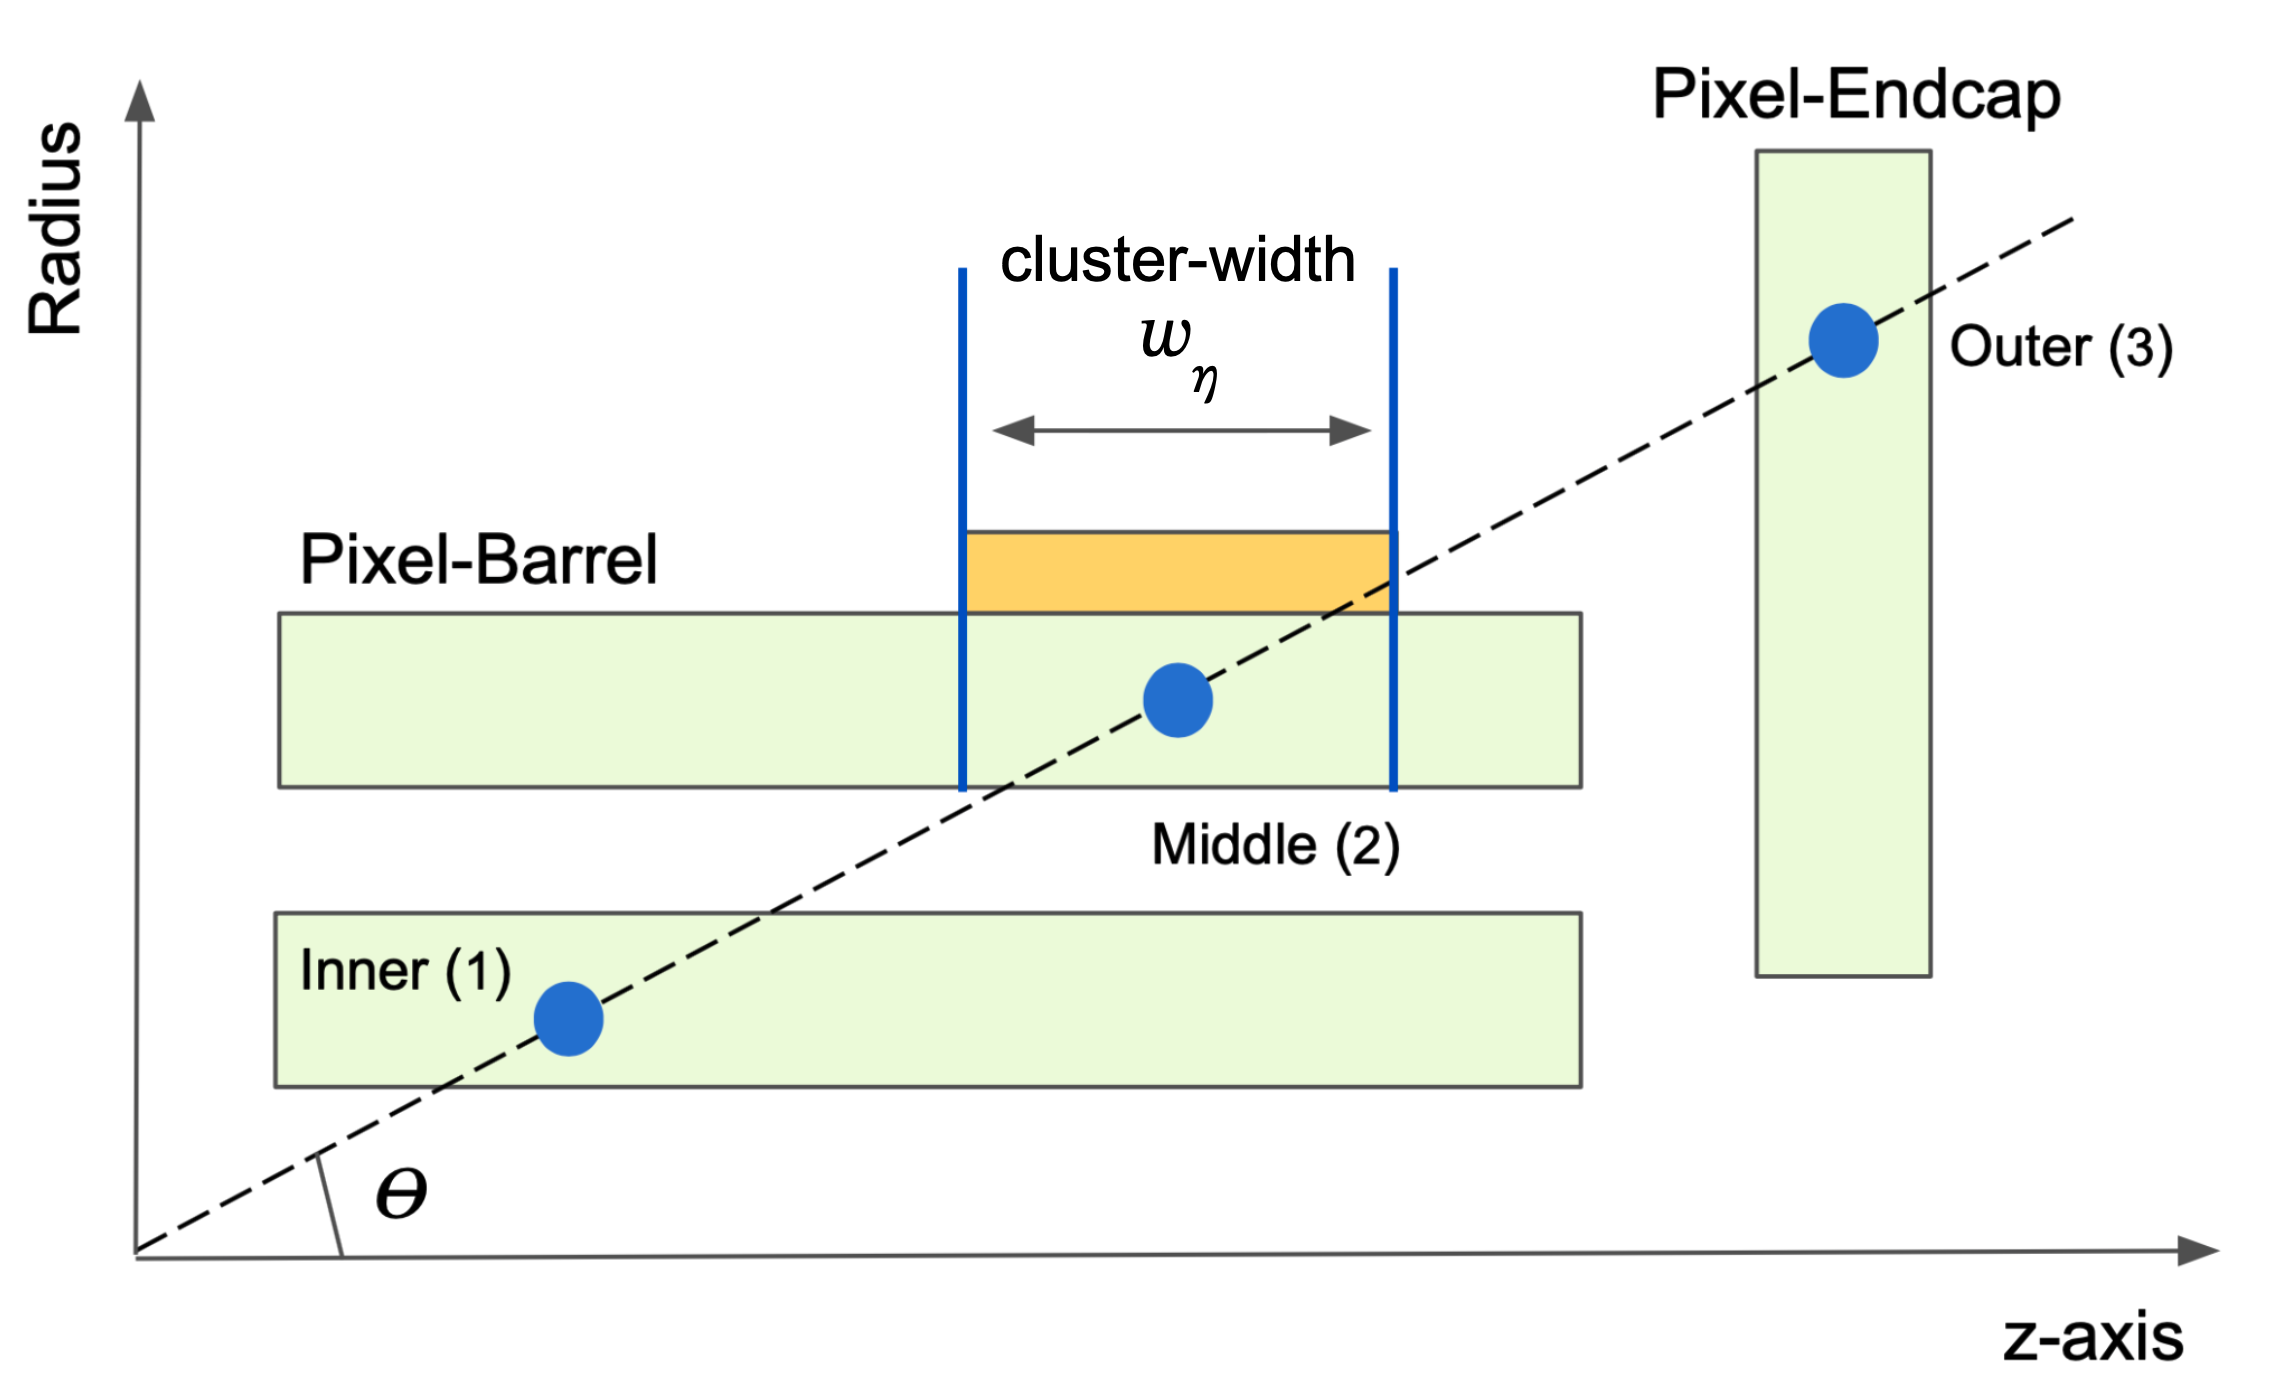
\includegraphics[width=0.85\linewidth]{images/4-ml-based-predictor/triplet_illustration_2.png}
    \caption{Seed illustration in the $r$-$z$ plane of the ID. The inner doublet consist of hits 1 and 2, and the outer doublet consist of hits 2 and 3. The longitudinal pixel-cluster width, $w_{\eta}$ (mm), is measured in the direction of $\eta$, where $\theta$ is the angle of inclination with respect to the $z$ axis.}
\label{fig:triplet-illustration}
\end{figure}


\subsection{Classifier Development}
\label{section:classifier-dev}

\subsubsection{Not-so-Naive Bayes}
% DONE

The basis of Bayes’ theorem \cite{naive-bayes} is used to build a classifier to discriminate between doublet classes, for both the pixel barrel and endcap regions. Bayesian analysis is based on having a prior probability of belief of an outcome of an event and a likelihood probability, where naive Bayes’ assumes that the conditional probabilities of the independent variables are statistically independent. The final classification is produced by computing the posterior probability by combining both the prior beliefs and the likelihood, which then determines the most probable class label. Using Bayes’ theorem is advantageous in this data-driven setting, as prior knowledge of the behaviour of the system is known. The posterior probability $P(c|x)$ that a given data point x belongs to class c is defined as:

\begin{equation} \label{naive-bayes}
    P(c|x) = \frac{P(x|c)P(c)}{P(x)}
\end{equation}

where $P(x|c)$ is the conditional likelihood, $P(c)$ is the class prior probability and $P(x)$ is the predictor prior probability, used for normalisation and calculated from the number of data points belonging to class $c$. Bayes' theorem is implemented using a generative model for each class. This was achieved by computing the likelihood function via a Kernel Density Estimate (KDE) for each of the 1-dimensional $|\cot(\theta)|$ distributions, forming a set of generative Bayesian classifiers. This method removes the 'naive' element and performs the same classification with a more sophisticated generative model for each class.

\subsubsection{Kernel Density Estimation}
% DONE

KDE is a non-parametric approach to estimate the probability density function of a random variable. The idea is that a kernel function is defined and centred on each data point in the sample. The sum of these functions together forms the kernel density estimate. The kernel density is defined as:
    
\begin{equation} \label{eq2}
    \hat{f}(x) = \frac{1}{Nh}  \sum_{i=1}^{N} K \left( \frac{x - x_i}{h} \right)
\end{equation}

where $K(x)$ is the kernel function, typically a smooth, symmetric and non-negative function, the kernel bandwidth $h$ controls the amount of smoothing applied to the function, where  $h > 0$ by definition and $N$ is the number of sample points used for normalisation \cite{kde}. One advantage of using KDE is that it provides a more flexible estimator parameterised by $h$. The KDE must be normalised in order to represent a probability density. For this study, the Gaussian kernel function was used to approximate the probability density at each data point in the sample. The area under a Gaussian curve is symmetrical, which is an appropriate regularisation. The Gaussian kernel is defined as:
    
\begin{equation} \label{eq3}
    K(x) = \frac{1}{\sqrt{2\pi}} e^{\frac{-x^2}{2}}
\end{equation}

The choice of bandwidth is important, as too large bandwidth results in a distribution where granular information is lost (over-smoothing). Conversely, a bandwidth that is too small, can lead to narrow peaks in close proximity to each other, resulting in a very noisy distribution (under-smoothing). There are several methods to determine the optimum bandwidth discussed in \cite{bandwidth-selection-methods}, many of which show similar properties. The method used in this study was the so-called \textit{Silverman's rule of thumb}, which works only for 1-dimensional data. Silverman's rule finds the bandwidth that minimizes the mean integrated squared error assuming that the data is Gaussian and a Gaussian kernel was used.

\newpage
\subsection{Classifier Training}
% DONE

The hit-pair data was separated into a training and a test dataset using a 70:30 split. The training data was analysed in the phase space of [$|\cot(\theta)|$, $w_{\eta}$]. Figure \ref{fig:truth-histo} shows an example of the 1-dimensional distributions of $|\cot(\theta)|$ for pixel barrel hit-pairs with $w_{\eta} \le$ 0.4 mm, where a clear distinction is observed between each truth class. The Bayes’ classifier was implemented in a generative way, computing the likelihood via a fitted KDE to each correct hit association distribution parameterised by $w_{\eta}$. The input feature vector, $\textbf{\textit{x}}$, comprised $|\cot(\theta)|$ and the truth label of the hit-pair formed the target output, $\textit{y}$. For unknown data points, the class which maximised the posterior was the class prediction.

After training, the predictions from each classifier were adjusted using the model's corresponding Receiver Operating Characteristic (ROC) curve \cite{Davis2006-oh}. The ROC curve indicates the performance of the classification model at all classification thresholds, where each point on the curve corresponds to a prediction probability. The ROC curve plots two parameters: True Positive Rate (TPR, also known as recall) and False Positive Rate (FPR), defined as:  

\begin{equation}
    TPR = \frac{TP}{TP + FN}, \quad FPR = \frac{FP}{FP + TN}
\end{equation}

where TP (True Positive) indicates the number of truth 1 hit-pairs correctly classified by the model and FN (False Negative) indicates the number of truth 1 hit-pairs incorrectly classified. In other words, TPR measures the proportion of positive instances correctly detected as positive by the model. Similarly, FP (False Positive) indicates the number of truth 0 hit-pairs incorrectly classified and TN (True Negative) indicates the number of truth 0 hit-pairs correctly classified. The TPR and FPR are two important performance metrics commonly used in binary classification problems to evaluate the effectiveness of a model to distinguish between the two classes. 

The ROC curve for the classifier is trained on the distribution for $w_{\eta} \le$ 0.4 mm is shown in Figure \ref{fig:roc-curve}. The classifier’s predictions were adjusted (also known as tuning) using the prediction probability derived from the ROC curve to yield a TPR of 0.95. Such a high TPR was chosen in order to maintain a high purity of correct hit-pairs. It is often more flexible to interpret probabilities than class predictions, as one is able to balance trade off concerns between FP prediction and FN prediction, and hence adjust thresholds.

The Area Under the Curve (AUC) represents a measure of separability and indicates the ability of a model to distinguish between classes. The value of the AUC is in the range 0.0 $\leq$ AUC $\leq$ 1.0, where AUC = 1 corresponds to perfect classification. The AUC achieved by the ML classifier for the $w_{\eta} \leq 0.4$ mm distribution was 0.79. The ‘no skill’ classifier with AUC = 0.5 is also shown in Figure \ref{fig:roc-curve}. This classifier cannot discriminate between correct or incorrect hit association classes and would predict a random class in all cases with 50\% probability.


\begin{figure}[htbp!] 
    \centering
    \subfloat[]{%
        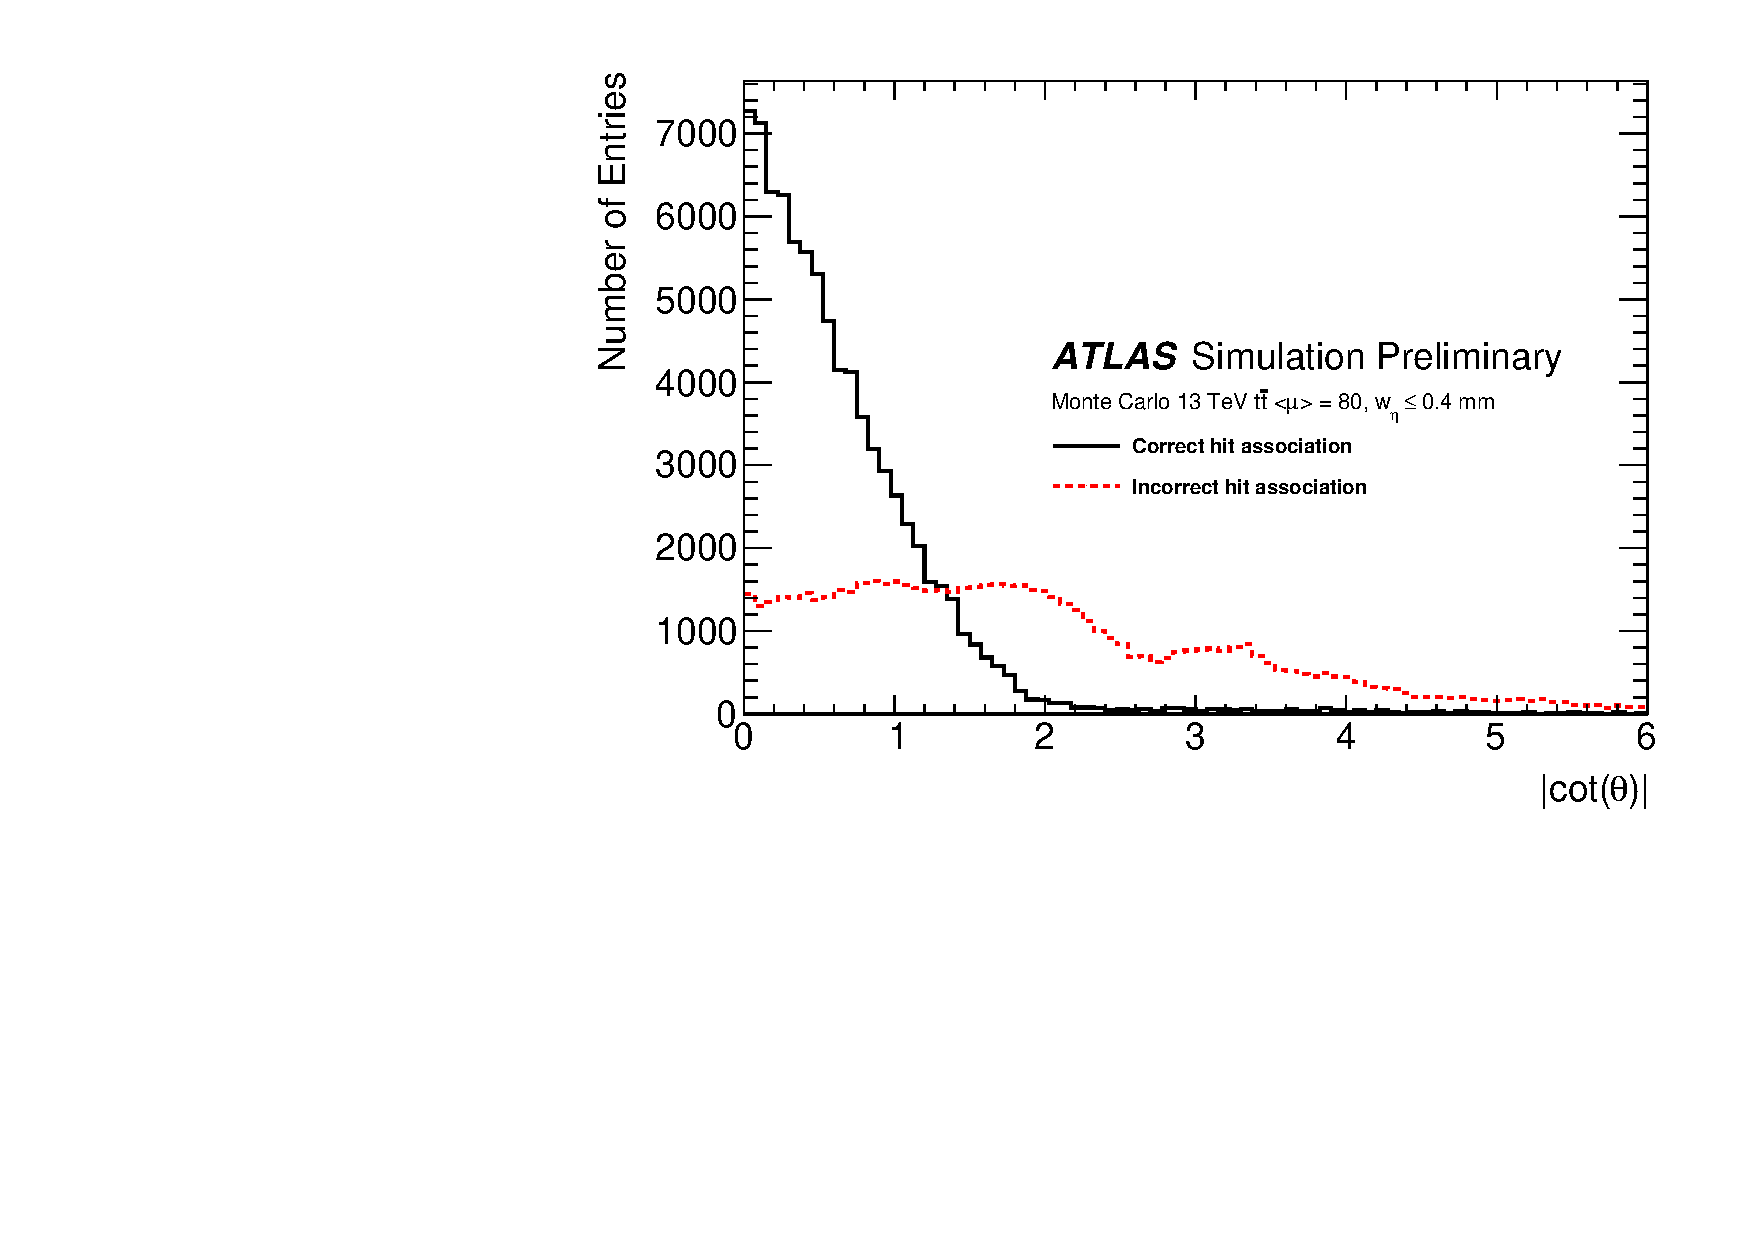
\includegraphics[width=0.98\textwidth]{images/4-ml-based-predictor/histo.pdf}%
        \label{fig:truth-histo}%
        }%
    \hfill%
    \subfloat[]{%
        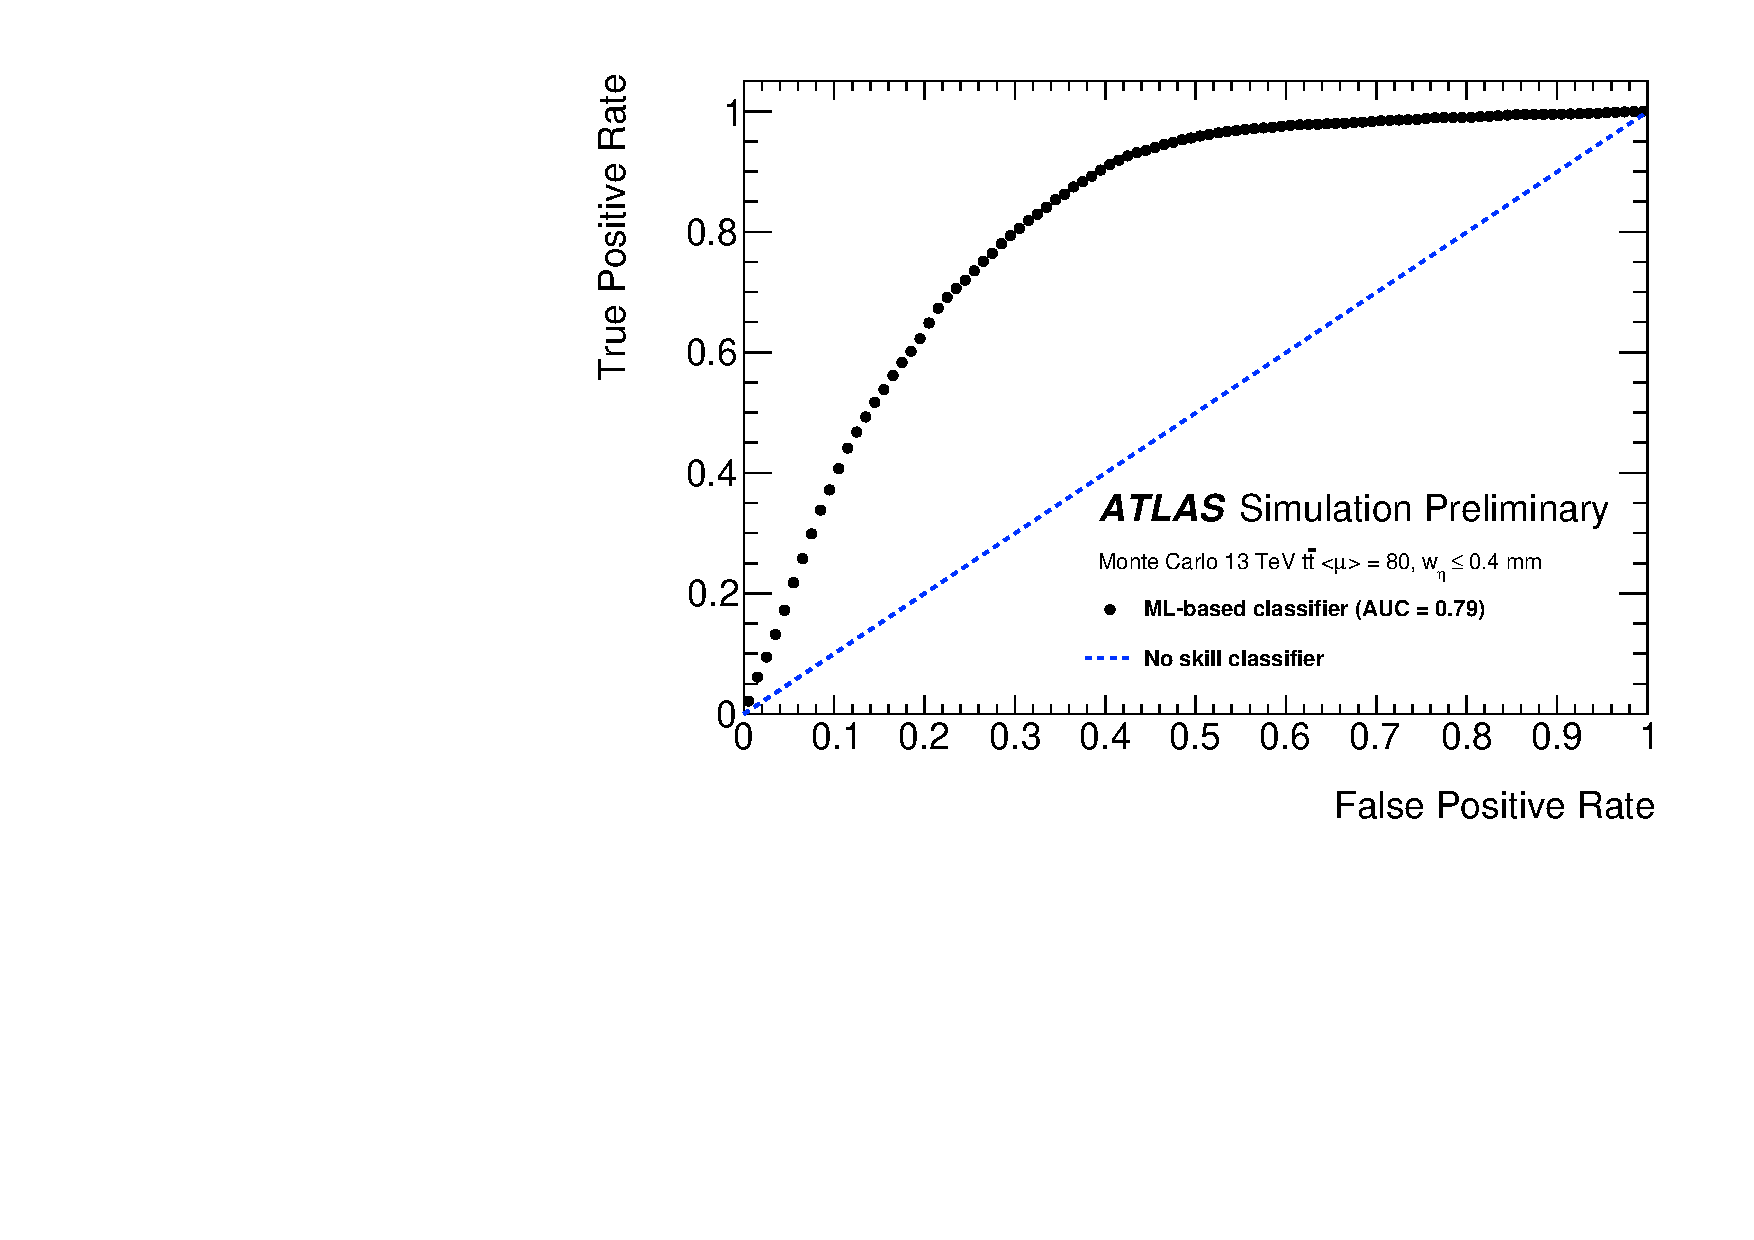
\includegraphics[width=0.98\textwidth]{images/4-ml-based-predictor/roc.pdf}%
        \label{fig:roc-curve}%
        }%
    \caption{(a) $\lvert \cot(\theta) \rvert$ for pixel barrel hit pairs with $w_{\eta} \leq 0.4$ mm in the ATLAS pixel detector, where $\theta$ is the inclination angle of the hit pair with respect to the $z$-axis. (b) The corresponding Receiver Operating Characteristic (ROC) curve for the classifier trained on the data shown in (a). The curve indicates the rates of false positive and true positive of pixel barrel hit pairs to tracks corresponding to truth particles.}
    \label{fig:1-dimensional-classifier-training}
\end{figure}


\subsubsection{Probability Calibration}

% READ THIS:
% https://machinelearningmastery.com/calibrated-classification-model-in-scikit-learn/
% https://scikit-learn.org/stable/modules/calibration.html

Probability calibration can provide more nuanced ways to evaluate the performance of the model. The discrepancies between the predicted probabilities of each classifier and its relative observed frequency for the positive class were analysed. A well calibrated model produces predictions that, on aggregate are closely aligned with the actual outcomes, and hence should appear as a diagonal. Points below the diagonal indicate a model is typically over-forecasting and conversely points above the diagonal indicate under-forecasting. There are several methods of probability calibration \cite{prob-calibration}. An Isotonic calibration fits a non-parametric regressor, whilst a Sigmoid calibration corresponds to a parametric approach. Each method was applied for the discrete 1-dimensional distributions. The performance was evaluated using the Brier score: the mean squared difference between the predicted probability and the actual outcome. Figure \ref{fig:calibration} shows the calibration curve of the classifier for the $w_{\eta} \leq 0.4$ mm distribution. Little difference was observed between the Brier score for the uncalibrated classifier and calibrated models. This was observed for all other 1-dimensional distributions in $w_{\eta}$. As a result, no additional probability calibration was applied during the development of the ensemble of KDE-based classifiers.

%KDE Calibration curve for pixel-barrel doublets with 0 - weta - 0.4. We can evaluate how well our model \& the predicted probabilities are calibrated. Calibration curve (reliability diagram) is generated for each weta bands, by analysing uncalibrated model, isotonic \& sigmoid calibration. Models are evaluated based on their Brier score (mean squared error). Uncalibrated KDE classifier (blue line) yields lowest error - no calibration needed

\begin{figure}[!htbp]
% \begin{figure}[htbp]
\centering
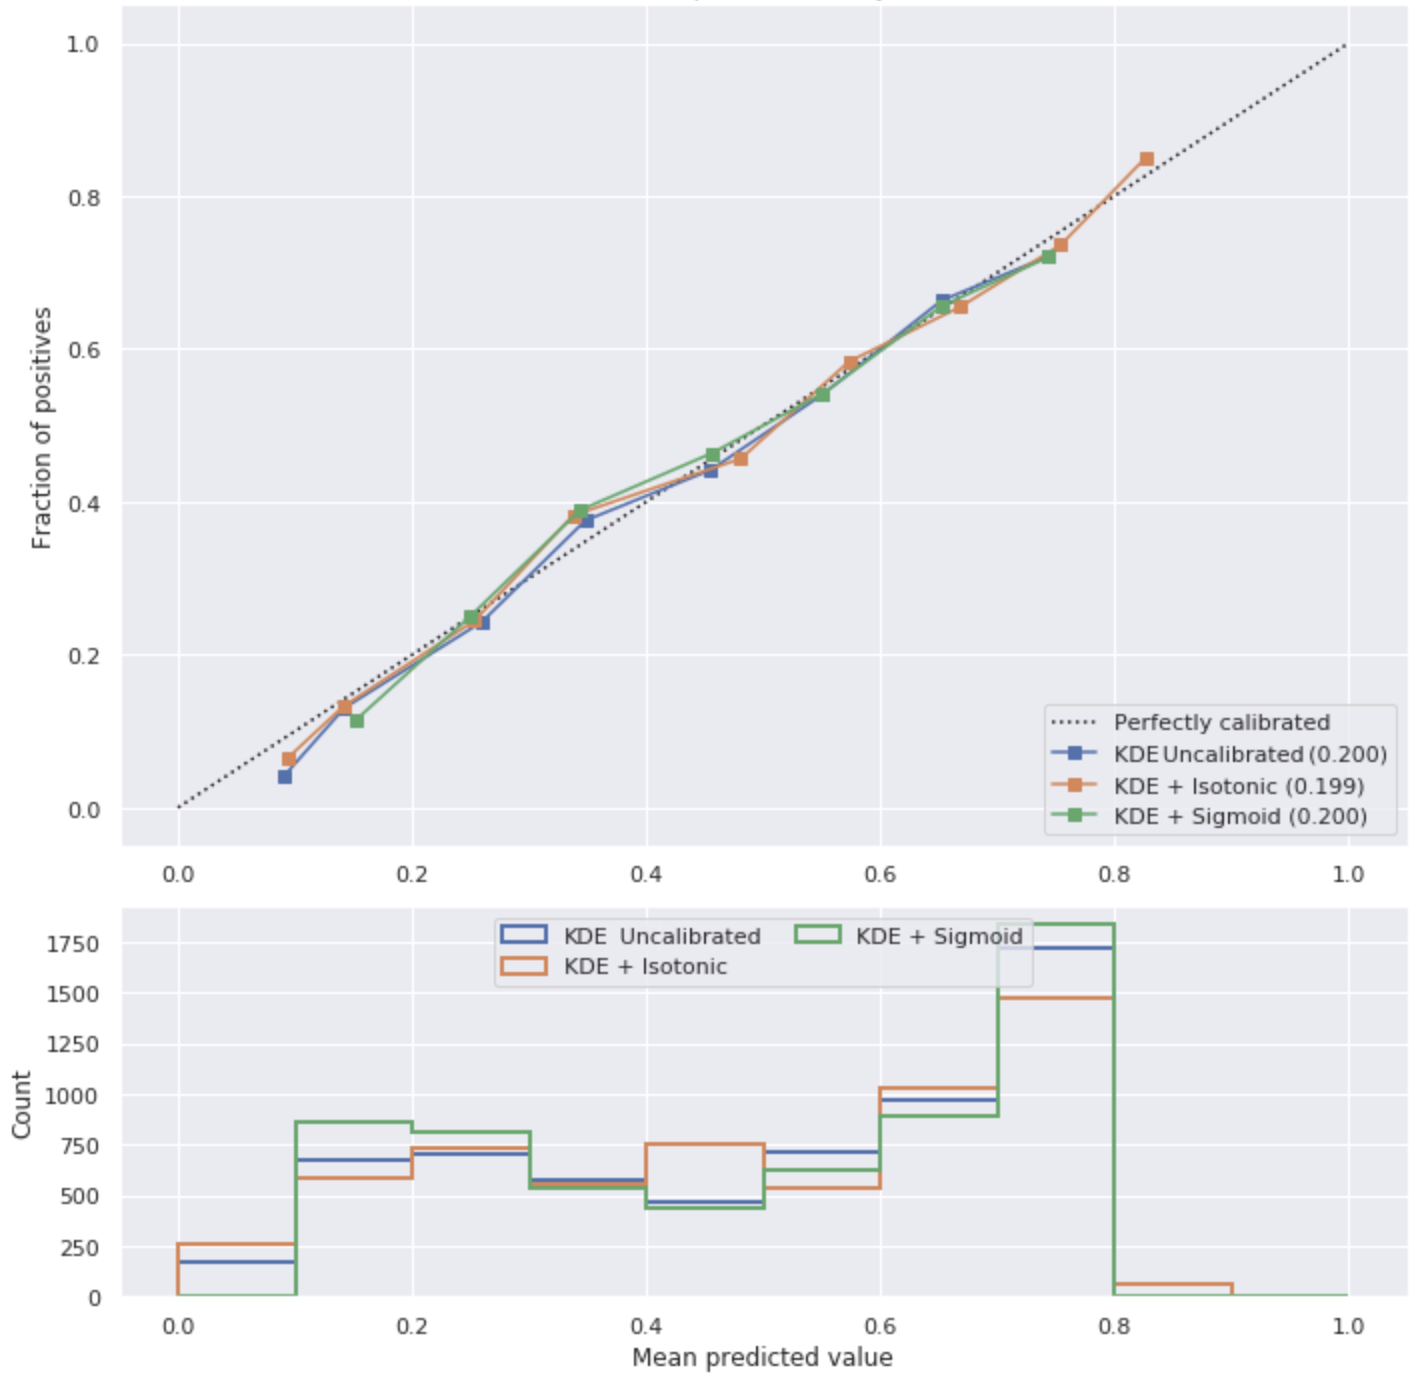
\includegraphics[width=1.0\linewidth]{images/4-ml-based-predictor/calibration2.png}
\caption{Reliability curve (top) for the KDE-based classifier predictions on pixel barrel hit-pairs with $ w_{\eta} \leq 0.4$ mm. Comparison of the uncalibrated KDE-based classifier with calibrated classifiers applied to the same training and test dataset. Common calibration techniques (Isotonic and Sigmoid functions) were tested. Models are evaluated based on their mean squared error, known as the Brier score quoted in the legend. The count for each distribution is also shown (bottom) as a function of mean predicted value.}
\label{fig:calibration}
\end{figure}


\subsection{Predictions and Evaluation}

Figure \ref{fig:predictions-pb-2d} shows the adjusted classifier predictions for pixel barrel hit-pairs after using the probability thresholds obtained from the corresponding ROC curves. A 2-dimensional acceptance-rejection region is observed; the black region of acceptance shows hit-pairs predicted with correct hit association. This follows a somewhat \textit{linear corridor} trend with a moving average as $w_{\eta}$ increases. Regions of hit-pair rejection are shown in red and fall into two main categories; the first are predicted to have low $w_{\eta}$ and large track inclination, the second predicted to have large $w_{\eta}$ and small track inclination. Overall, the recall achieved for hit-pairs with correct hit association was determined to be a tuned 95\%. Other metrics typically used within machine learning problems to evaluate the performance of classification models are the precision and F1 score defined as:


\begin{equation}
    Precision = \frac{TP}{TP + FP}, \quad F1 = \frac{2 \times precision \times recall}{precision + recall}
\end{equation}

where FP (False Positive) indicates the number of truth 0 hit-pairs incorrectly classified by the model and the recall is also known as the TPR. The precision refers to the the quality of the positive prediction made by the model, defined as the number of true positives divided by the total number of positive predictions. In other words, the precision provides the fraction of relevant instances among the retrieved instances. The F1 score combines the precision and recall into a harmonic mean. The precision achieved was 56\% and the F1 score achieved was 71\%. Typically, within ML algorithms one wants to optimize for either precision or recall, or find a balance between them. However, there is usually a trade-off between the two. In this study, there is greater importance in optimizing for the recall as this will allow for the prediction of FNs, and hence fakes, to be low.

% This is expected to originate from the forward region of the detector and....

For each classifier, the triplet selection efficiency and total seed rejection efficiency were evaluated, shown in Figure \ref{fig:predictions-pixel-barrel-and-triplet-efficiencies}. The seed selection efficiency is defined as the proportion of seeds with both its constituent doublets classified as correctly associated, out of all correctly associated seeds corresponding to MC truth from ATLAS tracking algorithms. This provides an indication of recall. The total seed rejection efficiency considers the proportion of rejected seeds, thereby providing an estimate of the total CPU time saved. This triplet validation stage provides an indication of the level of performance of the ML-based predictor directly on the seed building stage of the HLT tracking algorithm. The lower efficiency and corresponding reduced purity at $w_{\eta} \sim$ 2.0 mm is due to the transition between the barrel and endcap pixel detector layers. Overall, the seed selection efficiency achieved was 74.8 $\pm$ 0.1\% and the total seed rejection efficiency was 41.5 $\pm$ 0.1\%. This is primarily dominated by the low cluster width distribution ($w_{\eta} \leq$ 0.4 mm) where the greatest statistics is available for training data.


%The seed selection efficiency is defined as the proportion of seeds with both its constituent doublet pairs classified as correctly associated, out of all correctly associated seeds corresponding to MC truth from ATLAS tracking algorithms. and the total seed rejection efficiency considers the proportion of rejected seeds, thereby providing an estimate of the total CPU time saved. The lower efficiency and corresponding reduced purity around 2.0 mm is due to the transition between the barrel and endcap pixel detector. Errors shown here are purely statistical.


\begin{figure}[htbp!] 
    \centering
    \subfloat[]{%
        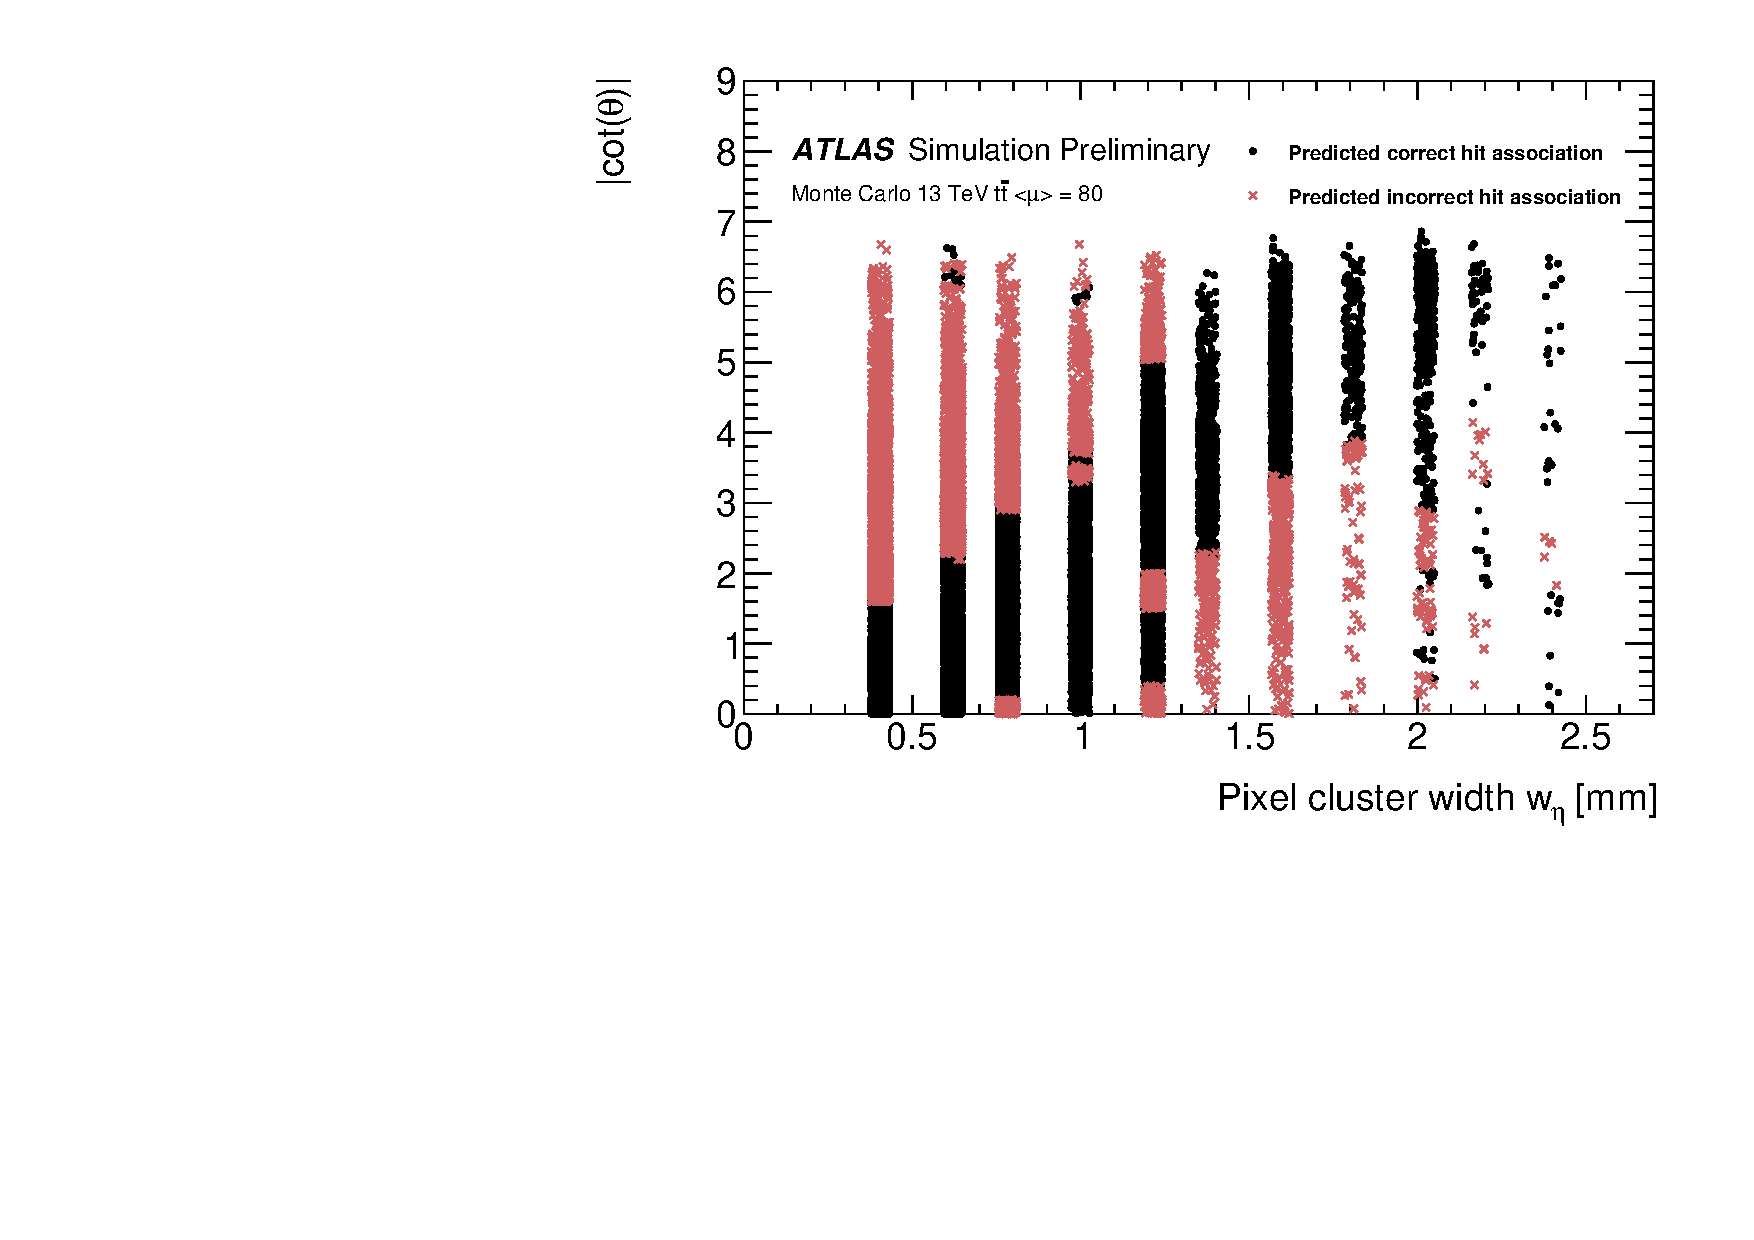
\includegraphics[width=0.98\textwidth]{images/4-ml-based-predictor/scatter_kde_predictions.pdf}%
        \label{fig:predictions-pb-2d}%
        }%
    \hfill%
    \subfloat[]{%
        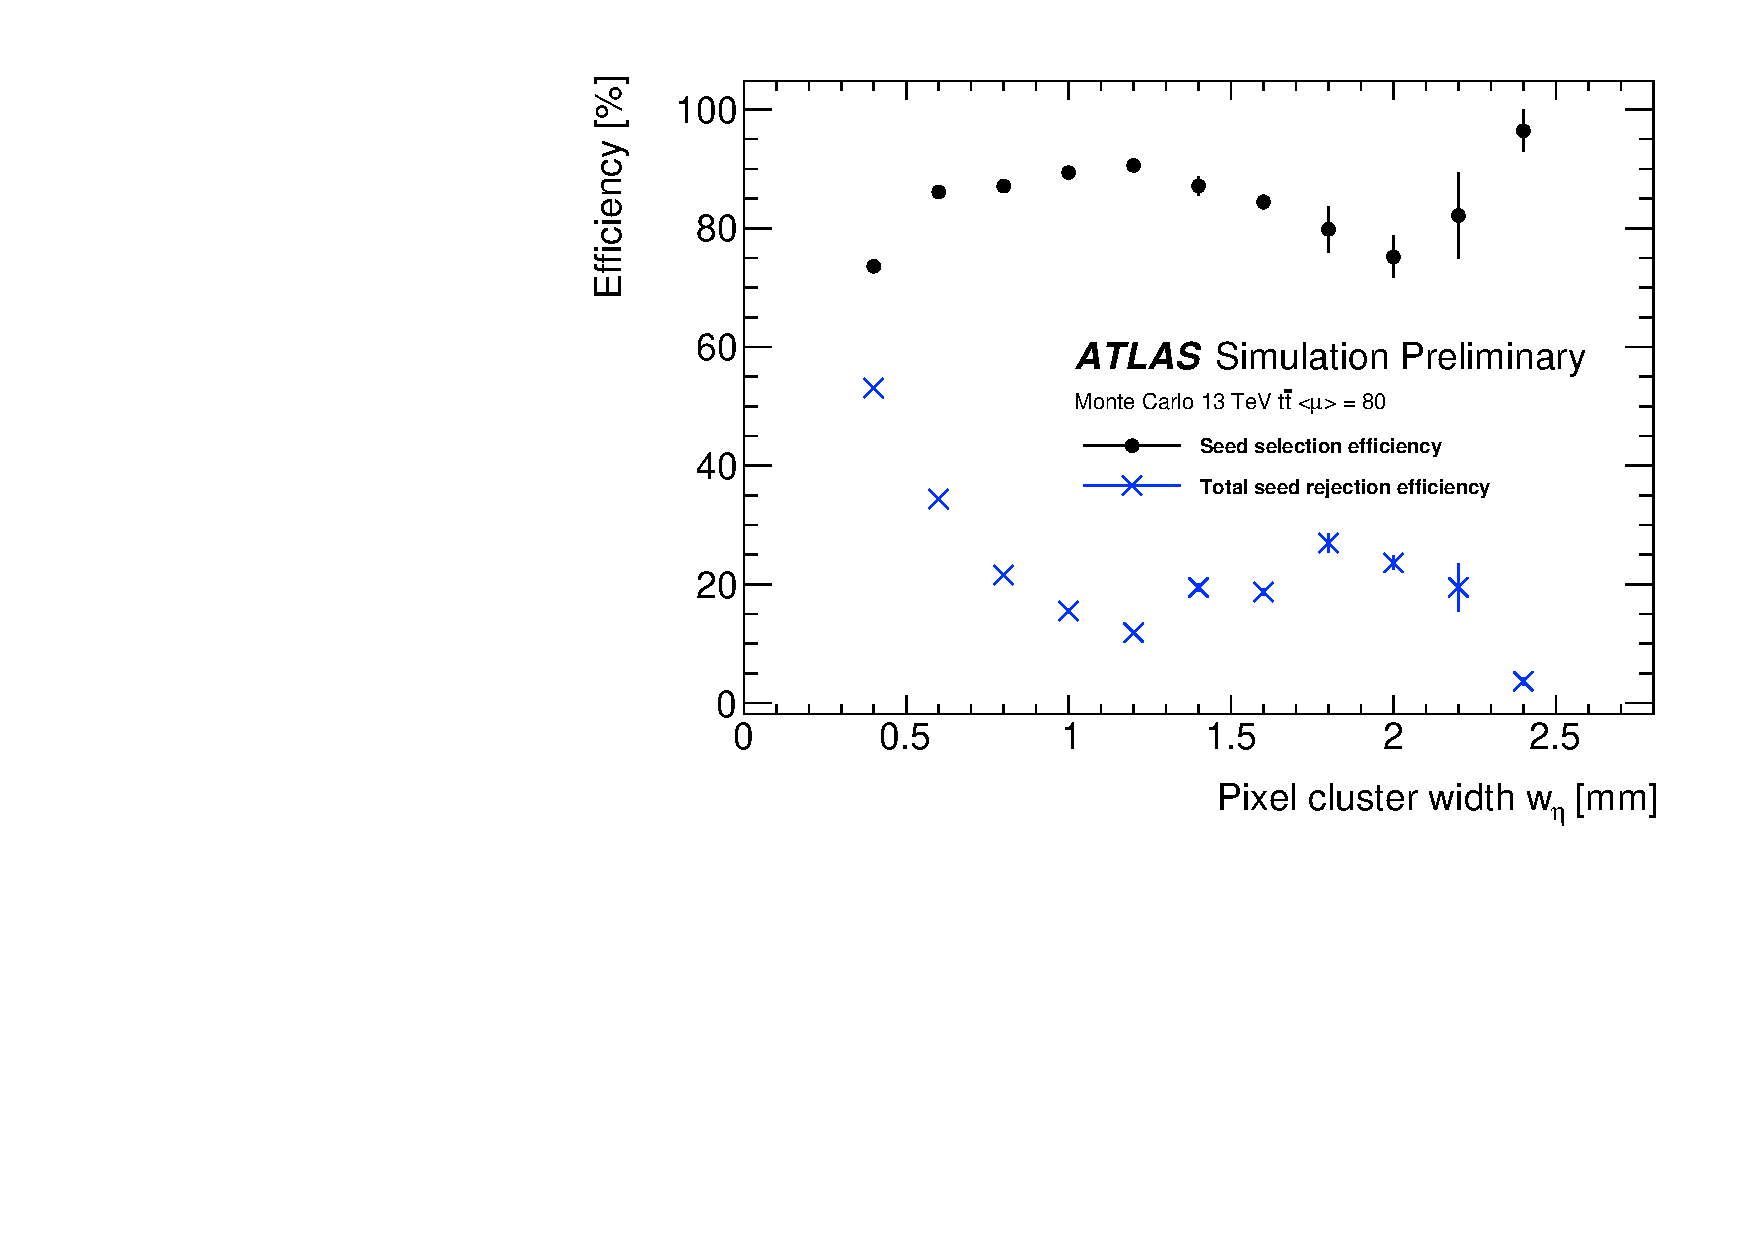
\includegraphics[width=0.98\textwidth]{images/4-ml-based-predictor/triplet_eff_metrics.pdf}%
        \label{fig:predictions-pixel-barrel-and-triplet-efficiencies}%
        }%
    \caption{(a) Predicted classification of pixel barrel hit pairs from the ATLAS pixel detector, trained using a set of ML classifiers to distinguish hit pairs matched to tracks corresponding to truth particles. Hit pair features used in training: $\lvert \cot(\theta) \rvert$, where $\theta$ is the inclination angle of the hit pair to the z-axis and the pixel cluster width $w_{\eta}$. The corresponding seed selection efficiency and total rejection efficiency are shown in (b). Errors shown here are purely statistical.}
\end{figure}





\section{Application of Hit-Pair Predictor}
\label{application-of-hit-pair-predictor}

\subsection{Look-Up Table Generation}
\label{LUT-generation}

Classifier predictions for the pixel regions were implemented directly into the ATLAS HLT \texttt{Fast Tracking} algorithm in the form of a Look-Up Table (LUT). This was achieved by first smoothing classifier predictions using Morphological filtering \cite{morphological-filtering} and then converting the acceptance region into a table. With reference to Figure \ref{fig:predictions-pb-2d} the predictions from classifiers $w_{\eta} > 2.0$ mm were not included in the morphological filtering, due to the low volume of statistics in this region. 

Morphological filtering is an image processing technique whereby non-linear transformations are applied to the binary matrix of an image, altering the features. Such non-linear operations include \texttt{dilation} and \texttt{erosion}. Dilation enlarges bright regions and shrinks dark regions, whereas erosion does the inverse of this. A combination of dilation and erosion was applied to the predictions made by the KDE-based classifiers for both the pixel barrel and endcap via rectangular structuring elements to achieve a smoothed structure. This was done in order to encourage horizontal extrapolation and elongation of the acceptance region.

The resulting acceptance region was converted into a binned LUT, the $w_{\eta}$ axes was divided into 45 bins between 0.0 - 3.0 mm and the $\lvert \cot(\theta) \rvert$ axes divided into 30 bins between 0.0 - 9.0, and the region to accept was recorded in the LUT. The bin values were chosen based on a heuristic choice, where the granularity of the acceptance region can be made stricter or looser depending upon the requirements and the degree of morphological filtering. A predefined LUT is a much more computationally efficient procedure than predicting class labels using a trained model. The LUT is fed directly into the \texttt{Fast Tracking} trigger algorithm, providing fast look-up to reduce computational overheads and the table itself is a very low cost option in terms of storage requirements. 



% \subsubsection{ML Filtering Modes}




\subsection{Performance Evaluation}
%DONE

The track reconstruction efficiency as a function of MC truth track $\eta$ and $p_T$ for the \texttt{Fast tracking} trigger stage are shown in Figure \ref{fig:efficiencies-ml-hit-pair-predictor}. The standard track seeding approach is compared with the application of ML filtering within the pixel detector. The standard seeding achieved an average tracking efficiency of 95\% with respect to MC truth tracks. The application of ML filtering at $\langle \mu \rangle$ = 80, achieved an average tracking efficiency of 93.9\%. The main loss in efficiency is observed at large $\lvert \eta \rvert$, due to the transition between the barrel and endcap pixel detector. This can be improved by generating greater statistics in this region within classifier training. Overall, there is little deviation in track reconstruction efficiency from the standard trigger seeding with application of ML extensions. In addition, there is an asymmetric nature in the efficiency as a function of $\eta$ observed in both the standard track seeding and track seeding with ML filtering in Figure \ref{fig:efficiencies-ml-hit-pair-predictor-eta}. One would expect a symmetric distribution due to the detector geometry. However, this is due to the alignment of the pixel modules being slightly rotated with respect to the z-axis. This type of geometry can precisely create this asymmetric effect.



\begin{figure}[htbp!] 
    \centering
    \subfloat[Efficiency vs. MC truth track $\eta$]{%
        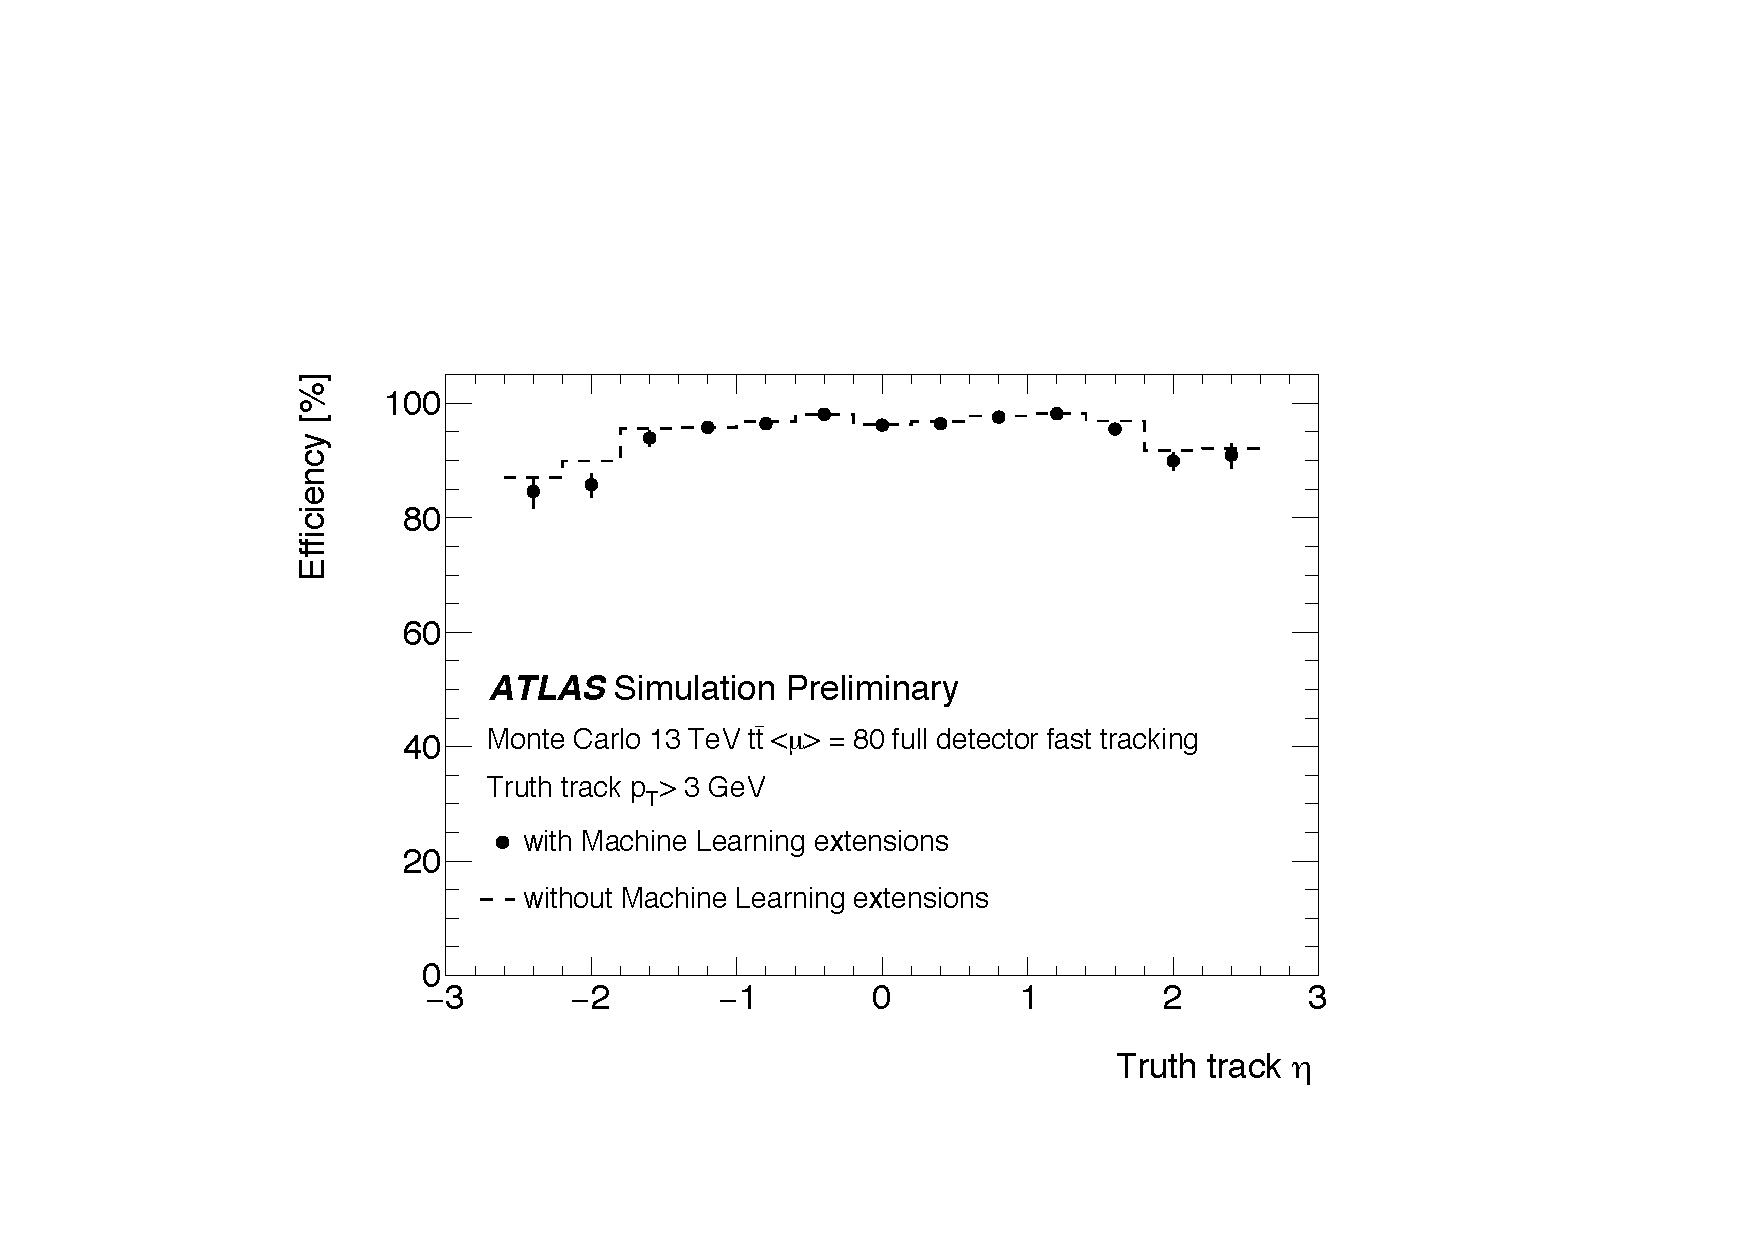
\includegraphics[width=0.92\textwidth]{images/4-ml-based-predictor/efficiency_eta.pdf}%
        \label{fig:efficiencies-ml-hit-pair-predictor-eta}%
        }%
    \hfill%
    \subfloat[Efficiency vs. MC truth track $p_{\mathrm{T}}$]{%
        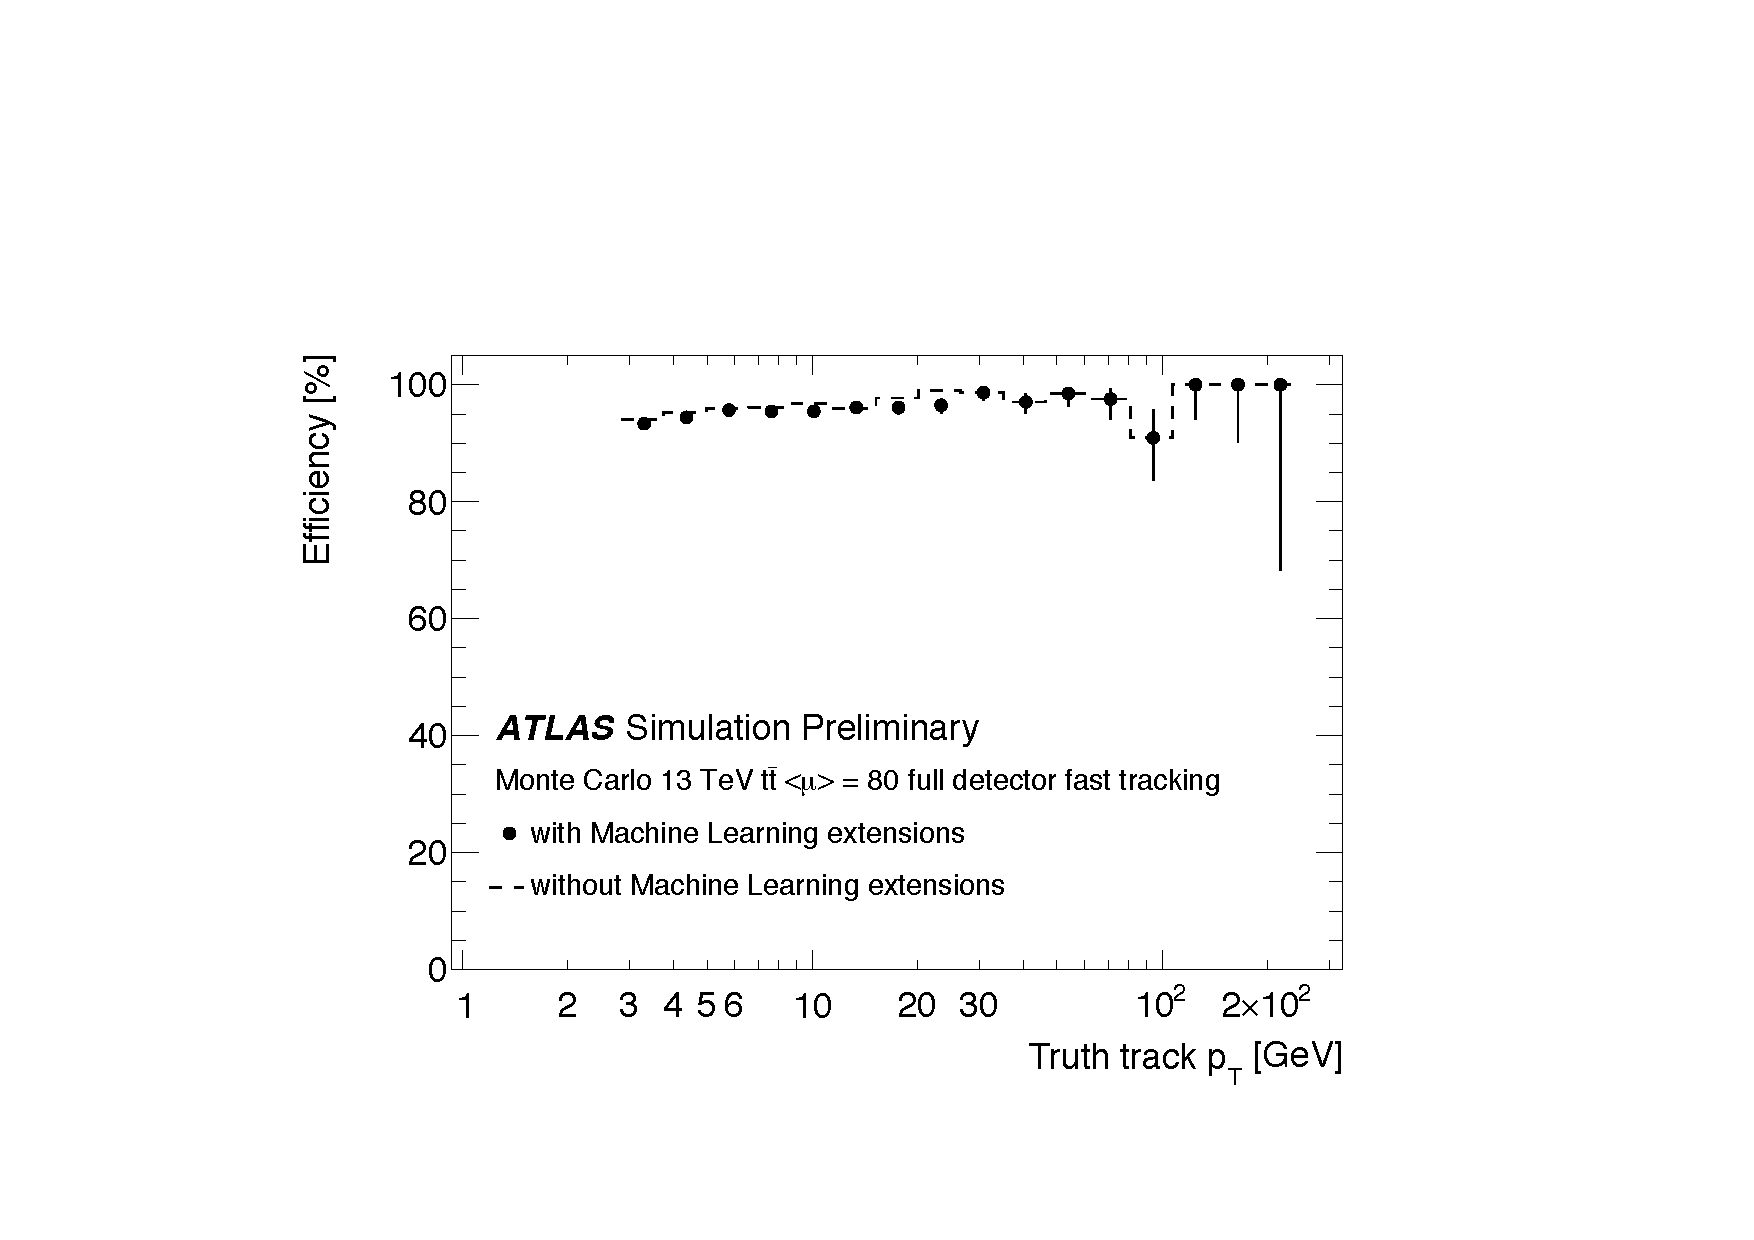
\includegraphics[width=0.92\textwidth]{images/4-ml-based-predictor/efficiency_pT.pdf}%
        \label{fig:efficiencies-ml-hit-pair-predictor-pt}%
        }%
    \caption{Tracking efficiencies as a function of track parameters, for $p_{T}$ > 3 GeV for the ATLAS full detector tracking with $t\overline{t}$ Monte Carlo 13 TeV and mean pile-up interaction multiplicity of $\langle \mu \rangle$ = 80. The data points show the efficiency when using machine learning extensions in the seed building stages of the fast tracking trigger in the ATLAS pixel detector, prior to the track fitting. The dashed line shows the efficiency of the standard trigger seeding with no application of machine learning extensions. The errors shown are purely statistical \cite{public-hlt}.}
    \label{fig:efficiencies-ml-hit-pair-predictor}
\end{figure}




\subsubsection{CPU Time Comparison}
% DONE

% TODO: know how the speed-up factor was measured - within an isolated testbed environment, with as little other processes occuring at the same time. Measuring the fastest time, and hence the greatest speed-up factor, not the average! - this is important here

Table \ref{tab:cpu} summarises the breakdown in speed-up factors achieved at various stages within the \texttt{Fast Tracking} trigger algorithm, with the application of the trained LUT for the pixel region. The total speed-up factor achieved in the full detector with application of ML extensions at $\langle \mu \rangle$ = 80 was observed to be 2.3. The greatest saving in CPU time is achieved during the \texttt{Seed Processing} stage, as a direct result of the significant reduction in the number of seeds. The average number of seeds processed for the standard tracking is $O(10^{4})$, whereas with the introduction of ML filtering for pixel seeds, approximately 78\% fewer seeds were selected for further processing. This significant reduction in CPU time does not only benefit the \texttt{Seed Processing} stage of the combinatorial track following algorithm in ATLAS, but also propagates to the \texttt{Track Fitting} stage.

\begin{table}[!htbp]
\caption{Performance of the ATLAS full detector tracking with MC 13 TeV $t\bar{t}$ samples at $\langle \mu \rangle = 80$, with the application of ML extensions for filtering on pixel detector hit-pairs in the \texttt{Fast Tracking} trigger stage \cite{public-hlt}. The total speed-up factor and breakdown of speed-ups at different stages of the \texttt{Fast Tracking} trigger algorithm are presented, each speed-up is presented with respect to the standard trigger seeding where no ML extensions are applied.}
\begin{center}
\begin{tabular}{llll}
\toprule
Total Speed-up Factor & Seed Generation & Seed Processing & Track Fitting \\
\hline
2.3 & 1.3 & 3.3 & 1.5 \\ 
\bottomrule
\end{tabular}
\end{center}
\label{tab:cpu}
\end{table}

\subsubsection{Changing Pile-up Conditions}
% DONE

Table \ref{tab:pileup} summarises the relative efficiency loss and relative speed-up factor, with application of ML extensions for the ATLAS pixel detector for various $\langle \mu \rangle$, presented with respect to the standard trigger seeding, where no ML extensions were applied. A general trend is observed whereby the speed-up factor increases as $\langle \mu \rangle$ increases. At $\langle \mu \rangle$ = 80, the loss in track reconstruction efficiency was observed to be 1.1\%, which was acceptable by the ID trigger performance requirements at the time of writing.


\begin{table}[!htbp]
\caption{Performance of the ATLAS full detector tracking with MC 13 TeV $t\bar{t}$ samples at $\langle \mu \rangle$ = 40, 60 and 80, with the application of ML extensions for filtering on pixel detector hit-pairs in the \texttt{Fast Tracking} trigger stage\cite{public-hlt}. The absolute loss in average tracking efficiency and the total speed-up factor for seeded track finding are presented with respect to the standard trigger seeding where no ML extensions were applied. The efficiency loss is mainly observed at large $|\eta|$. The statistical uncertainties in efficiencies are $O(10^{-3})$, hence are not quoted.}
\begin{center}
\begin{tabular}{ccc}
\toprule
$\langle \mu \rangle$ & Efficiency Loss (\%) & Total Speed-up Factor  \\
\hline
40 & 0.7 & 1.6 \\
60 & 0.7 & 2.1 \\
80 & 1.1 & 2.3 \\
\bottomrule
\end{tabular}
\end{center}
\label{tab:pileup}
\end{table}


\section{Other Approaches}
\subsection{Multiple Acceptance Regions}
% DONE

When training on varying permutations of train and test data sets, a second acceptance region was frequently predicted for the 1-dimensional distributions where pixel barrel hit-pairs possess low cluster width and high track inclination. This second region is highlighted in Figure \ref{fig:multiple-acceptance} which shows the KDE-based classifier's predictions for a particular train-test permutation. The hit-pairs predicted as belonging to class 1 having correct hit association for $w_{\eta} = 0.6$ mm and $w_{\eta} = 1.0$ mm appear at the tail ends of these distributions. These hits were isolated and their local cluster position in the $\eta$ direction was analysed. Approximately 60\% of hits possessed the largest absolute local cluster position and this was observed for each occurrence of a second acceptance region appearing at low cluster-width and high track inclination. This corresponds to hits being located at the extremes of the barrel module, since their dimensions are approximately 20 mm $\times$ 60 mm \cite{pixel-module-dimensions} and strongly suggests that the second acceptance region had originated from module edge pixels. Further investigation would be needed in order to handle these space-points separately. One reason for separate handling of these space-points is that morphological smoothing is applied uniformly to an image, hence any dilation may interact with the general shape of the main acceptance region and would increase the proportion of fakes accepted.

\begin{figure}[!htbp]
% \begin{figure}[htbp]
\centering
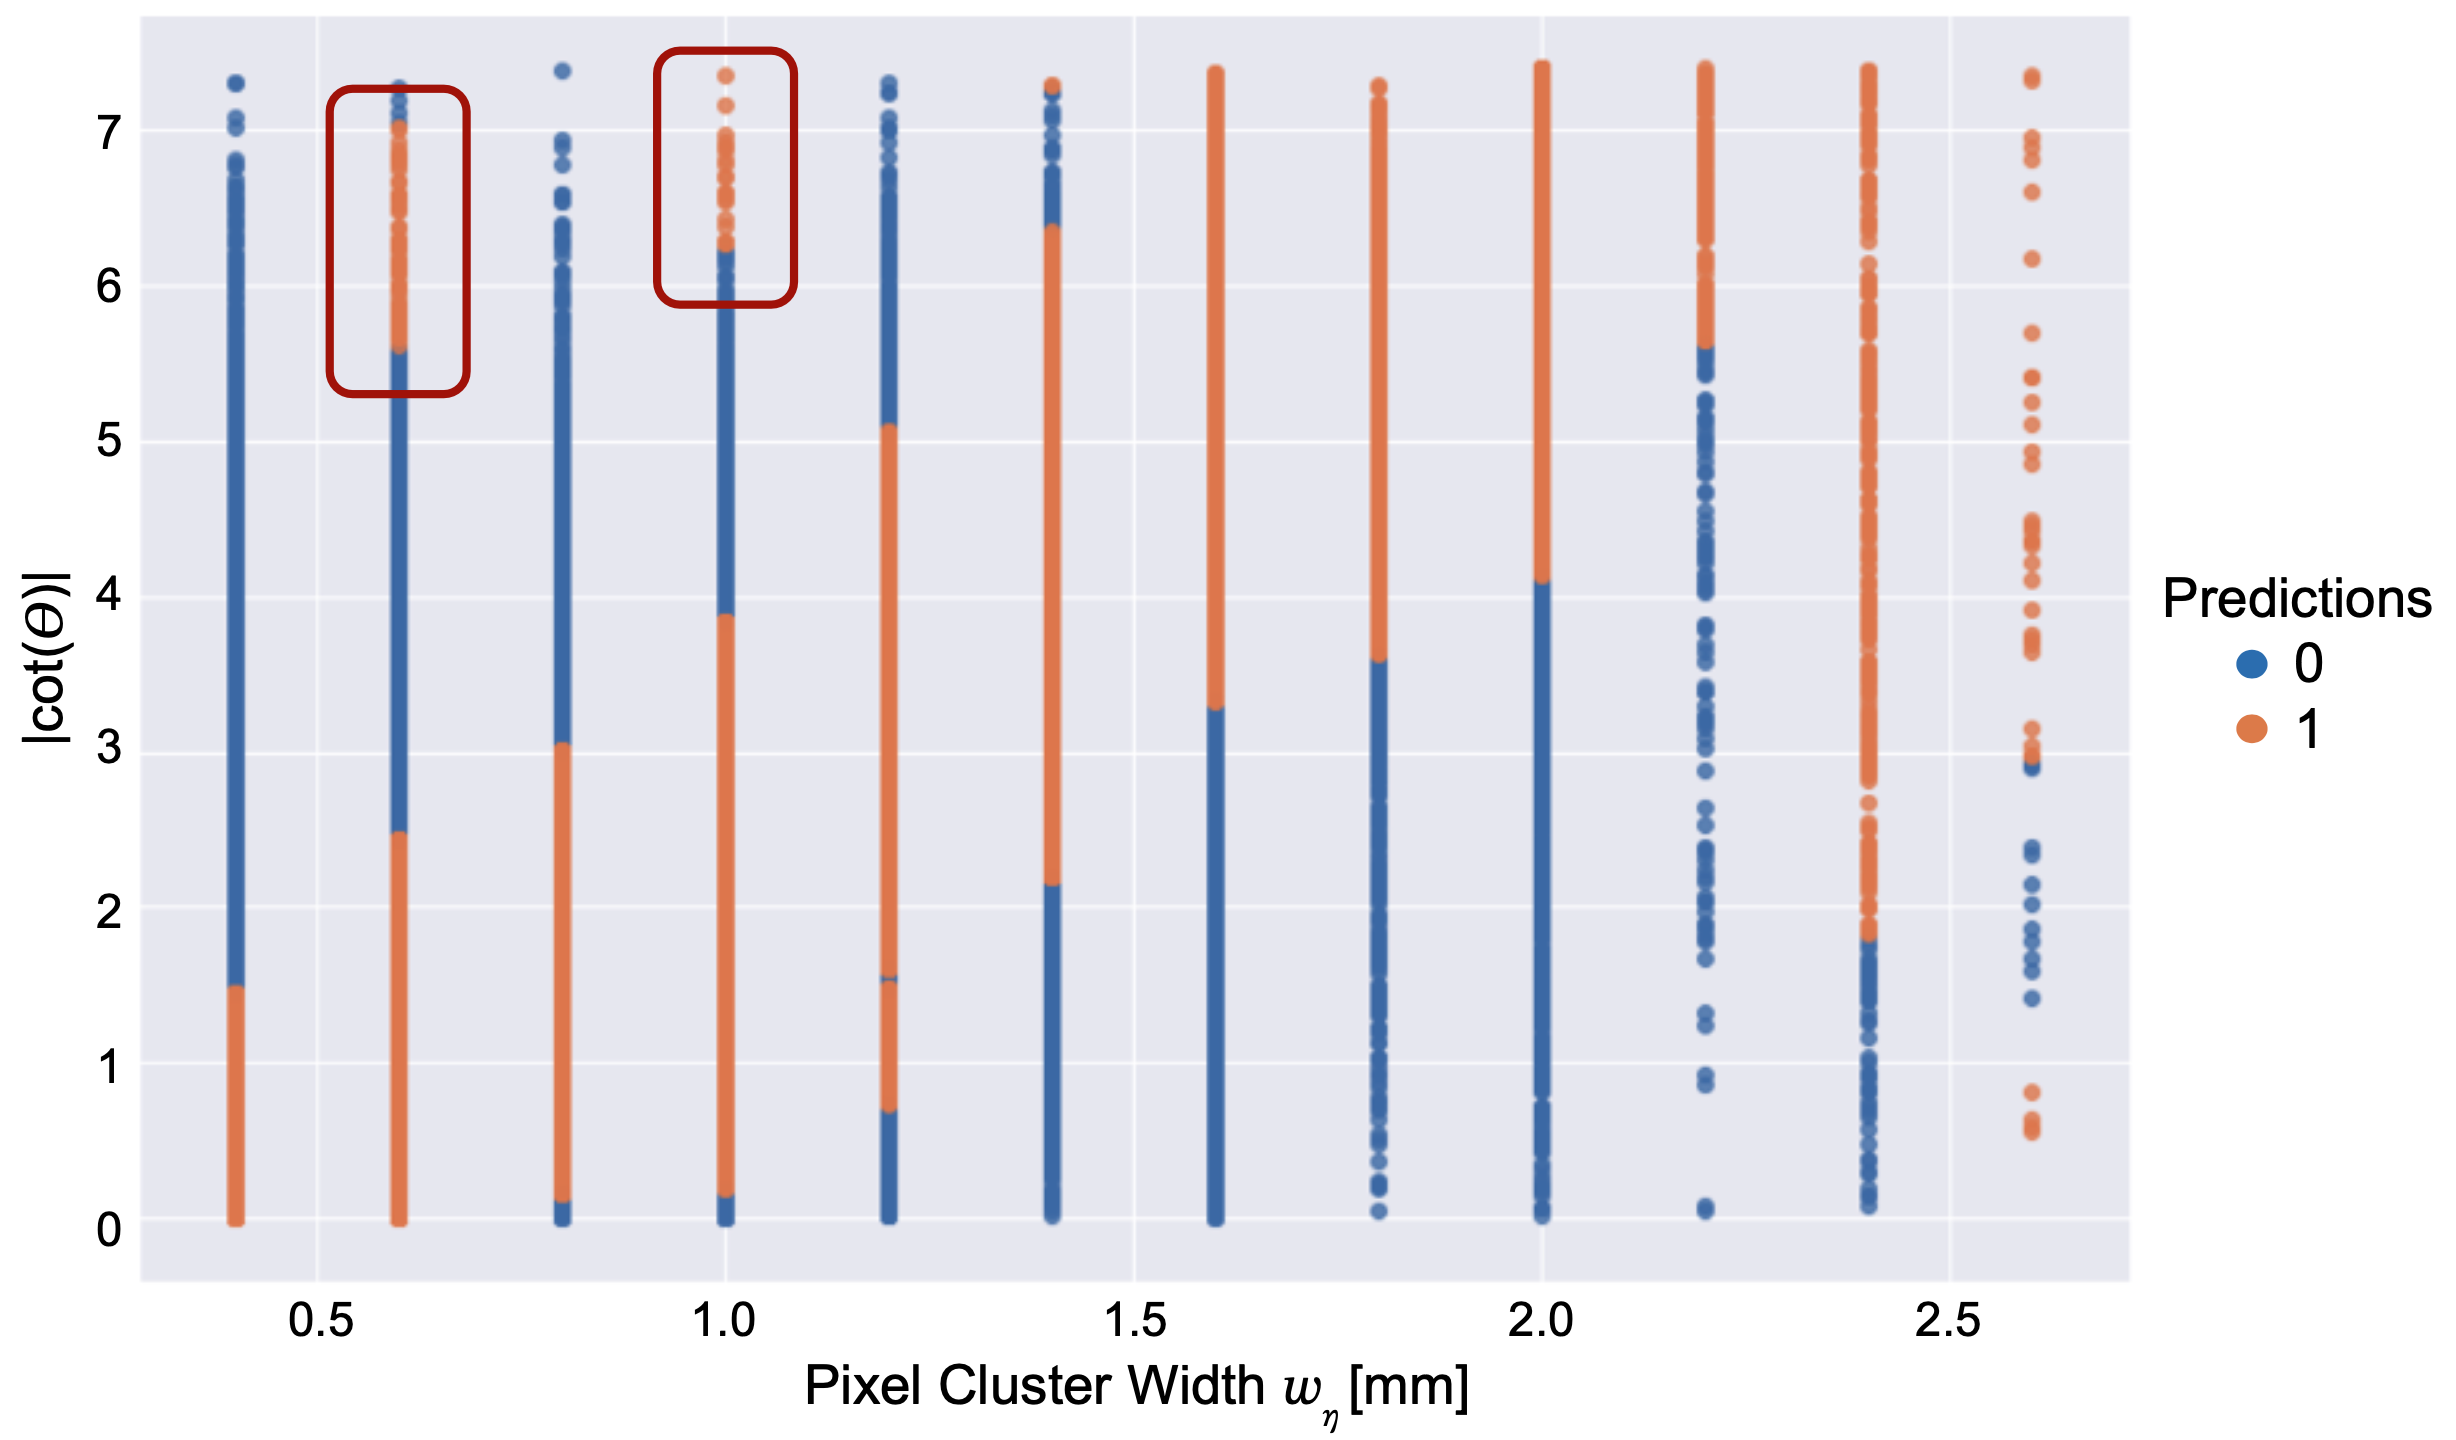
\includegraphics[width=0.98\linewidth]{images/4-ml-based-predictor/Multiple_acceptance_regions.png}
\caption{KDE-based classifier predictions for the pixel barrel hit pairs. Multiple acceptance regions are observed at large track inclination for $w_{\eta} = 0.6$mm and $w_{\eta} = 1.0$mm, circled in red.}
\label{fig:multiple-acceptance}
\end{figure}


\subsection{Support Vector Machine}
% DONE

% See this website for further explanation 
% https://towardsdatascience.com/support-vector-machine-introduction-to-machine-learning-algorithms-934a444fca47
% multi class classification: one-to-rest
% https://towardsdatascience.com/multiclass-classification-with-support-vector-machines-svm-kernel-trick-kernel-functions-f9d5377d6f02

Another supervised learning algorithm investigated was the Support Vector Machine (SVM) \cite{svm}. The objective of a SVM is to find a hyperplane (known as a decision boundary) in a N-dimensional space (where N is the number of features) that distinctly classifies the data points and is typically used in binary classification. The optimal decision boundary is one which maximizes the margins between the two classes. This provides some reinforcement that unseen data points can be classified with more confidence. For non-linear decision boundaries, the SVM uses the so-called \textit{kernel trick} to project the data into a higher dimensional space to find a plane where the data is linearly separable. 

The SVM was applied to the data in the phase space of  [$|\cot(\theta)|$, $w_{\eta}$]. However in this instance the observed discrete nature affected the mechanics of the classifier and its ability to determine a decision boundary. Therefore, a prior step to training the SVM was to apply Principal Component Analysis (PCA). PCA is commonly used as a dimensionality reduction technique \cite{pca}, however here it was applied to remove the ordinal nature of the cluster widths which introduces a systematic bias to the SVM kernel. By doing so, the data was transformed into a continuous 2-dimensional phase space, where the variance of the truth 1 class is maximal along the first principal component axis. A hyperparameter sweep of various kernels was executed using cross-validation and the polynomial kernel of third degree with hyperparameters $C=0.75$ and $\gamma=0.05$, was found to produce the highest TPR of 95\%. Hyperparameter $C$ is a regularization parameter, such that a greater $C$ would result in a smaller margin being accepted. This essentially behaves as a penalty term and controls the cost of misclassification. Hyperparameter $\gamma$ controls the distance of influence of a single training point. The predictions of the PCA-SVM classifier on pixel barrel data and the corresponding decision boundary are shown in Figure \ref{fig:barrel-svm-pca}. The shaded orange-red region indicates predicted hit-pairs with correct association, whereas the shaded blue region indicates predicted hit-pairs with incorrect association.

By applying a combination of PCA and SVM, the classifier was able to separate the two classes well. However, the corresponding FPR obtained was 82\% and the ROC AUC was 0.53, very similar to the no-skill classifier. Both of these metrics indicate that a large proportion of hit-pairs were incorrectly accepted by the model and hence this would increase the proportion of fake seeds constructed by downstream algorithms.

% \begin{figure}[!htbp]
\begin{figure}[htbp]
\centering
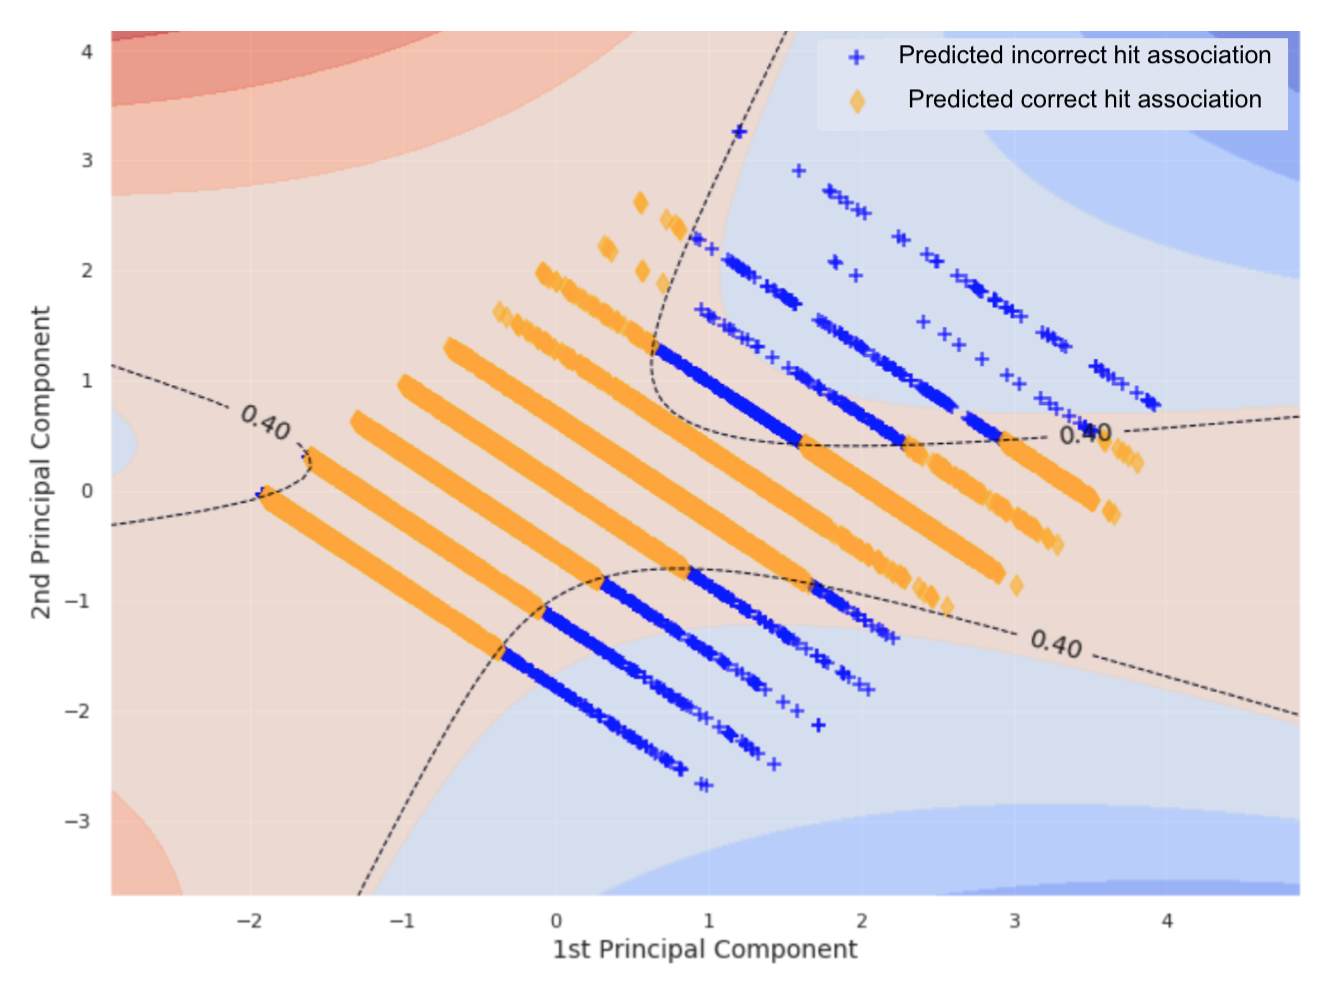
\includegraphics[width=1.0\linewidth]{images/4-ml-based-predictor/barrel-svm-pca.png}
\caption{PCA transform and SVM classifier applied to pixel barrel hit pairs. The SVM decision boundary predictions are illustrated, where the black dotted line represents the threshold value of 0.40 yielding a TPR of 95\%. Predicted hit-pairs with correct association are illustrated by diamonds (orange) and predicted hit pairs with incorrect association are illustrated with + (blue). The SVM kernel used for the classifier was a polynomial degree 3 kernel with hyperparameters $C=0.75$ and $\gamma=0.05$. The 1st principal component indicates the axis of largest variance within the class with correct hit association doublet class.}
\label{fig:barrel-svm-pca}
\end{figure}

SVMs generally perform well, even when trained with imbalanced data sets. This, coupled with the fact that a distinct decision boundary could be easily extracted and converted into a LUT, would lead to less ambiguity in comparison to applying an extrapolation using morphological smoothing. However, there are key disadvantages by using a SVM rather than Bayes' theorem in this instance. The probabilistic information contained within each discrete one-dimensional distribution of $w_{\eta}$ is lost, which is an important feature when tuning each individual distribution. Additionally, the SVM typically fits a continuous function for the decision boundary and hence may not be strict enough in certain regions. This factor is important when considering the proportion of fake seeds being accepted using a LUT generated from such a decision boundary. Due to these key differences in classifiers, this method was not pursued further.


\subsection{Comparison with Deep Learning Approaches}

%algorithms share common approaches and methods

An algorithm with similar functionality to the method presented in this chapter, is that of the solution submitted to the TrackML competition known as \textit{Outrunner} \cite{Amrouche_2019}. The Outrunner algorithm uses a deep neural network model composed of multiple wide hidden layers and is trained to predict the adjacency matrix of hits, i.e. the probability of a hit-pair to be on the same track, in an all-to-all network connection scheme. This approach is an unstructured track following algorithm where the next hit is not provided by track extrapolation but directly by a hit index based on the hit pair classifier score. The proposed solution is prohibitively expensive for track candidate prediction, due to the extremely high combinatorics of hit pairs that are followed, yet the method is highly accurate. In contrast, the classical ML method presented in this chapter achieves the same result for hit-pair prediction without the need for high compute resources. The Outrunner algorithm also uses a LUT input approach of classifier predictions, as this provides the fastest inference and implementation for a realistic detector.

%The proposed approach is an unstructured track following algorithm where the next hit is not provided by track extrapolation but directly a hit index based on the hit pair classifier score. The reported prohibitive computation cost seems to indicates that much too many branches of the combinatorial tree are followed during the track following step. Some level of tuning could result in similar performance without much loss of accuracy, and may constitute an alternative the the combinatorial track finder approach. Although the proposed solution is prohibitively expensive to be used for making track candidate prediction, it is rather accurate, and further development might make it much more tractable. It should be noted that graph based neural network approaches, such as the one presented in [20] can combine the hit pair classification and the navigation of the adjacent hits.

% comparison with ExaTrkX project:
Additionally, the ML-based predictor developed in this chapter can also be compared to the graph construction method used by Exa.TrkX. The Exa.TrkX collaboration also predict compatible edge connections by a metric learning approach. This comprises a deep learning technique by training a MLP to learn pixel cluster features, such as space-point position, the direction of the hit-pair and the dimensions of the module. Each node in the MLP is embedded into a N-dimensional latent space, which is a hugely CPU intensive task. The goal of this task is similar to the approach developed in this chapter, however they differ in their implementation. Deep learning is not used in this case, instead a Bayesian KDE-based classifier is employed. The main difference here is that within the procedure developed by Exa.TrkX, training is required each time as predictions have not been converted into a LUT, putting a large strain on computational resources. Whereas, in the methodology in this chapter proposes an alternative technique utilising traditional ML approaches which are less CPU intensive.


\section{Conclusion}
%DONE

As the luminosity and collision rate increases during future upgrades of the LHC program, novel and precise tracking methodologies, as well as efficient use of computing power will become increasingly important in the selection of physics objects. Therefore, it is essential that resource use is reduced, whilst maintaining the ability to reconstruct tracks with minimal efficiency loss. 

The work presented in this chapter demonstrates the algorithms and techniques implemented to optimise the HLT ID track seeding software for ATLAS Run-3 and beyond, in order to reduce the number of fake track seeds. The ML-based algorithm developed is used to predict if a pair of hits belong to the same track given input hit features of pixel cluster width and inverse track inclination. It is encouraging to see that the application of the ML-based classifier for seed selection in the ATLAS ID has provided significant CPU savings on trained MC data at various pile-up levels. The trained predictor in the form of a LUT yields 2.3$\times$ speed-up with a 1.1\% loss in track reconstruction efficiency at $\langle \mu \rangle$ = 80, compared with the standard trigger tracking. The developed ML pipeline is advantageous for many reasons. It provides a flexible way to generate custom LUTs depending on the degree of efficiency required; the predictor can be trained to yield a desired TPR. This ML setup can be used to generate custom LUTs for different geometrical setups, isolating different requirements for the barrel and endcap regions, as well as for particular decay signatures depending on the required efficiency. It is useful to have algorithms that allow movement to different working points of efficiency vs CPU time, as this allows one to optimise the trigger depending on the requirements. The fast lookup implementation bodes well in a realistic detector setup. The handling of doublets which have their inner hit located in the barrel layer and their outer hit located in the endcap layer can be revisited to try to improve the performance in the transition region. Additionally, increasing statistics of the generation of hit-pairs would improve the accuracy in the prediction of incompatible doublets, particularly for regions with $w_{\eta} > 2$ mm. Overall, the reduction in fakes at an earlier stage in the HLT track seeding, ensures the reduction of fake seed propagation into downstream tracking stages and allows significant savings in CPU resources.

%i.e. jets, the training would need to be done again specifically for that purpose.

%. The use of different ML filtering modes applied to the triplets, can produce varying efficiencies (and speed up), where the three least redundant combinations are presented in this study. Additionally, proper training and tuning of the classifier can yield a required TPR, therefore allowing the flexibility in strictness.
